%%%%%%%%%%%%%%%%%%%%%%%%%%%%%%%%%%%%%%%%%
% cuRAMSES-kjhan Technical Reference Manual
%%%%%%%%%%%%%%%%%%%%%%%%%%%%%%%%%%%%%%%%%

%----------------------------------------------------------------------------------------
%    PACKAGES AND OTHER DOCUMENT CONFIGURATIONS
%----------------------------------------------------------------------------------------

\documentclass[11pt,fleqn]{book}

\usepackage[top=3cm,bottom=3cm,left=3.2cm,right=3.2cm,headsep=10pt,headheight=14pt,a4paper]{geometry}

\usepackage{xcolor}
\definecolor{ocre}{RGB}{52,177,201}

% Font Settings
\usepackage{avant}
\usepackage{mathptmx}
\usepackage{microtype}
\usepackage[utf8]{inputenc}
\usepackage[T1]{fontenc}

% Bibliography
\usepackage[style=alphabetic,sorting=nyt,sortcites=true,autopunct=true,hyperref=true,abbreviate=false,backref=true,backend=biber]{biblatex}
\addbibresource{bibliography.bib}
\defbibheading{bibempty}{}

%%%%%%%%%%%%%%%%%%%%%%%%%%%%%%%%%%%%%%%%%
% Modern Software Documentation Style
% Custom design for cuRAMSES-kjhan
% tcolorbox-based environments
%%%%%%%%%%%%%%%%%%%%%%%%%%%%%%%%%%%%%%%%%

%----------------------------------------------------------------------------------------
%	REQUIRED PACKAGES
%----------------------------------------------------------------------------------------

\usepackage{graphicx}
\usepackage{tikz}
\usetikzlibrary{calc}

\usepackage{enumitem}
\setlist{nolistsep}

\usepackage{booktabs}
\usepackage{longtable}
\usepackage{array}
\newcolumntype{L}[1]{>{\raggedright\arraybackslash}p{#1}}
\newcolumntype{C}[1]{>{\centering\arraybackslash}p{#1}}
\newcolumntype{R}[1]{>{\raggedleft\arraybackslash}p{#1}}

\usepackage{amsmath,amsfonts,amssymb,amsthm}
\usepackage{etoolbox}

\usepackage{makeidx}
\makeindex

%----------------------------------------------------------------------------------------
%	ADDITIONAL COLORS
%----------------------------------------------------------------------------------------

\colorlet{darkocre}{ocre!70!black}
\definecolor{codebg}{RGB}{245,247,250}
\definecolor{codeframe}{RGB}{200,210,220}
\definecolor{darkblue}{RGB}{0,51,102}
\definecolor{successgreen}{RGB}{39,174,96}
\definecolor{dangered}{RGB}{192,57,43}

%----------------------------------------------------------------------------------------
%	CODE LISTINGS
%----------------------------------------------------------------------------------------

\usepackage{listings}
\lstset{
    basicstyle=\ttfamily\small,
    backgroundcolor=\color{codebg},
    frame=single,
    rulecolor=\color{codeframe},
    breaklines=true,
    numbers=left,
    numberstyle=\tiny\color{gray},
    keywordstyle=\color{darkocre}\bfseries,
    commentstyle=\color{successgreen!70!black}\itshape,
    stringstyle=\color{dangered},
    showstringspaces=false,
    tabsize=4,
    xleftmargin=2em,
    framexleftmargin=1.5em,
    aboveskip=1em,
    belowskip=1em
}

\lstdefinestyle{fortran}{
    language=[95]Fortran,
    morekeywords={integer,real,logical,character,allocatable,intent,
    dimension,implicit,none,use,module,contains,subroutine,function,
    end,call,if,then,else,endif,do,enddo,return,include,kind,dp,i8b,
    save,present,optional,select,case,type,class}
}

\lstdefinestyle{bash}{
    language=bash,
    morekeywords={make,mpirun,cd,cp,nohup,export}
}

%----------------------------------------------------------------------------------------
%	PAGE HEADERS
%----------------------------------------------------------------------------------------

\usepackage{fancyhdr}
\pagestyle{fancy}
\fancyhf{}
\fancyhead[LE,RO]{\sffamily\normalsize\thepage}
\fancyhead[LO]{\sffamily\small\nouppercase{\rightmark}}
\fancyhead[RE]{\sffamily\small\nouppercase{\leftmark}}
\renewcommand{\headrulewidth}{0.4pt}
\renewcommand{\headrule}{\hbox to\headwidth{%
    \color{ocre!50}\leaders\hrule height \headrulewidth\hfill}}
\renewcommand{\footrulewidth}{0pt}
\fancypagestyle{plain}{\fancyhead{}\renewcommand{\headrulewidth}{0pt}}

%----------------------------------------------------------------------------------------
%	CHAPTER AND SECTION HEADINGS
%----------------------------------------------------------------------------------------

\usepackage[explicit]{titlesec}

% Chapter: large number + colored rule
\titleformat{\chapter}[display]
    {\normalfont\sffamily\bfseries}
    {\flushright\fontsize{80}{90}\selectfont\color{ocre!20}\thechapter}
    {-1.5cm}
    {\flushright\color{darkocre}\Huge#1}
    [\vspace{0.3em}{\color{ocre}\titlerule[2pt]}]

\titleformat{name=\chapter,numberless}[display]
    {\normalfont\sffamily\bfseries}
    {}
    {-0.5cm}
    {\color{darkocre}\Huge#1}
    [\vspace{0.3em}{\color{ocre}\titlerule[2pt]}]

\titlespacing*{\chapter}{0pt}{-20pt}{30pt}

% Section
\titleformat{\section}
    {\normalfont\Large\bfseries\sffamily\color{darkocre}}
    {\color{ocre}\thesection}{0.5em}{#1}

% Subsection
\titleformat{\subsection}
    {\normalfont\large\bfseries\sffamily}
    {\color{ocre}\thesubsection}{0.5em}{#1}

% Subsubsection
\titleformat{\subsubsection}
    {\normalfont\normalsize\bfseries\sffamily}
    {\color{ocre}\thesubsubsection}{0.5em}{#1}

% Part
\titleformat{\part}[display]
    {\centering\normalfont\huge\bfseries\sffamily\color{darkocre}}
    {\fontsize{80}{90}\selectfont\color{ocre!20}\thepart}
    {1em}
    {\Huge#1}
    [\vspace{0.5em}{\color{ocre}\titlerule[3pt]}]

%----------------------------------------------------------------------------------------
%	TABLE OF CONTENTS
%----------------------------------------------------------------------------------------

\usepackage{titletoc}
\contentsmargin{0cm}

\titlecontents{part}[0cm]
    {\addvspace{20pt}\centering\large\bfseries\sffamily}
    {\color{ocre}\thecontentslabel\quad}
    {}
    {}

\titlecontents{chapter}[1.25cm]
    {\addvspace{12pt}\large\sffamily\bfseries}
    {\color{ocre}\contentslabel[\Large\thecontentslabel]{1.25cm}\color{darkocre}}
    {\color{darkocre}}
    {\color{ocre}\normalsize\;\titlerule*[.5pc]{.}\;\thecontentspage}

\titlecontents{section}[1.25cm]
    {\addvspace{3pt}\sffamily\bfseries}
    {\contentslabel[\thecontentslabel]{1.25cm}}
    {}
    {~\titlerule*[.5pc]{.}~\thecontentspage}

\titlecontents{subsection}[1.25cm]
    {\addvspace{1pt}\sffamily\small}
    {\contentslabel[\thecontentslabel]{1.25cm}}
    {}
    {~\titlerule*[.5pc]{.}~\thecontentspage}

%----------------------------------------------------------------------------------------
%	COLORED ENVIRONMENTS (tcolorbox)
%----------------------------------------------------------------------------------------

\usepackage[most]{tcolorbox}
\tcbuselibrary{skins,breakable}

% Definition
\newtcolorbox[auto counter,number within=chapter]{definition}[1][]{%
    enhanced,breakable,
    colback=ocre!5,
    colframe=ocre,
    coltitle=white,
    fonttitle=\bfseries\sffamily,
    title=Definition~\thetcbcounter\ifstrempty{#1}{}{~(#1)},
    attach boxed title to top left={yshift=-2mm,xshift=5mm},
    boxed title style={colback=ocre,sharp corners,boxrule=0pt},
    sharp corners,
    boxrule=0.5pt,
    left=5pt,right=5pt,top=8pt,bottom=5pt
}

% Theorem
\newtcolorbox[auto counter,number within=chapter]{theorem}[1][]{%
    enhanced,breakable,
    colback=darkblue!5,
    colframe=darkblue!80,
    coltitle=white,
    fonttitle=\bfseries\sffamily,
    title=Theorem~\thetcbcounter\ifstrempty{#1}{}{~(#1)},
    attach boxed title to top left={yshift=-2mm,xshift=5mm},
    boxed title style={colback=darkblue!80,sharp corners,boxrule=0pt},
    sharp corners,
    boxrule=0.5pt,
    left=5pt,right=5pt,top=8pt,bottom=5pt
}

% Example
\newtcolorbox[auto counter,number within=chapter]{example}[1][]{%
    enhanced,breakable,
    colback=successgreen!5,
    colframe=successgreen!70!black,
    coltitle=white,
    fonttitle=\bfseries\sffamily,
    title=Example~\thetcbcounter\ifstrempty{#1}{}{~(#1)},
    attach boxed title to top left={yshift=-2mm,xshift=5mm},
    boxed title style={colback=successgreen!70!black,sharp corners,boxrule=0pt},
    sharp corners,
    boxrule=0.5pt,
    left=5pt,right=5pt,top=8pt,bottom=5pt
}

% Remark (left-ruled, blue)
\newtcolorbox{remark}[1][Remark]{%
    enhanced,breakable,
    colback=darkblue!3,
    colframe=darkblue,
    coltitle=darkblue,
    fonttitle=\bfseries\sffamily,
    title=#1,
    boxrule=0pt,
    leftrule=4pt,
    sharp corners,
    left=5pt,right=5pt,top=5pt,bottom=5pt
}

% Info box (left-ruled, teal)
\newtcolorbox{infobox}[1][Info]{%
    enhanced,breakable,
    colback=ocre!5,
    colframe=ocre,
    coltitle=darkocre,
    fonttitle=\bfseries\sffamily,
    title=#1,
    boxrule=0pt,
    leftrule=4pt,
    sharp corners,
    left=5pt,right=5pt,top=5pt,bottom=5pt
}

% Important (left-ruled, red)
\newtcolorbox{important}{%
    enhanced,breakable,
    colback=dangered!5,
    colframe=dangered,
    coltitle=dangered!90!black,
    fonttitle=\bfseries\sffamily,
    title=Important,
    boxrule=0pt,
    leftrule=4pt,
    sharp corners,
    left=5pt,right=5pt,top=5pt,bottom=5pt
}

% Code box (simple wrapper — compatible with lstlisting inside)
\newenvironment{codebox}[1][]{%
    \par\medskip
    \ifstrempty{#1}{}{{\noindent\sffamily\small\bfseries\color{darkocre}#1}\par\nobreak\vspace{-0.8em}}%
}{%
    \par\medskip
}

%----------------------------------------------------------------------------------------
%	HYPERLINKS
%----------------------------------------------------------------------------------------

\usepackage{hyperref}
\hypersetup{
    colorlinks=true,
    linkcolor=darkocre,
    citecolor=darkblue,
    urlcolor=ocre,
    bookmarks=true,
    bookmarksopen=false
}


%----------------------------------------------------------------------------------------
%    Definitions of new commands
%----------------------------------------------------------------------------------------

\def\R{\mathbb{R}}

%------------------------------------------------------
% Document
%------------------------------------------------------
\begin{document}

%------------------------------------------------------
% Title page
%------------------------------------------------------
\begin{titlepage}

\begin{tikzpicture}[remember picture,overlay]
  % Top colored area
  \fill[ocre] (current page.north west) rectangle ([yshift=-9cm]current page.north east);
  % Bottom accent strip
  \fill[ocre!10] (current page.south west) rectangle ([yshift=2.5cm]current page.south east);
  \draw[ocre,line width=1.5pt] ([yshift=2.5cm]current page.south west) -- ([yshift=2.5cm]current page.south east);
\end{tikzpicture}

\vspace*{1cm}

\begin{center}
{\fontsize{42}{50}\selectfont\sffamily\bfseries\color{white}cuRAMSES-kjhan}\\[1cm]
{\fontsize{20}{24}\selectfont\sffamily\color{white!80}Technical Reference Manual}
\end{center}

\vspace{5cm}

\begin{center}
{\Large\sffamily
K-Section Ordering, Morton Key Octree,\\[8pt]
Memory-Based Load Balancing, and\\[8pt]
Performance Optimizations}

\vspace{3cm}

{\large\sffamily Juhan~Kim}\\[0.5cm]
{\sffamily February 2026}
\end{center}

\vfill

\begin{center}
{\small\sffamily
Based on RAMSES (R.~Teyssier)\\[3pt]
\texttt{git@github.com:kjhan0606/cuRAMSES-kjhan.git}}
\end{center}
\vspace{1cm}
\end{titlepage}

%------------------------------------------------------
% Table of Contents
%------------------------------------------------------

\pagestyle{empty}
\tableofcontents
\pagestyle{fancy}

%------------------------------------------------------
% PART I: Modifications Overview
%------------------------------------------------------
\part{Code Modifications}

%======================================================
\chapter{Quick Start Guide}
\label{ch:quickstart}
%======================================================

This chapter provides a practical step-by-step guide to building cuRAMSES and running a cosmological zoom-in simulation. For detailed explanations of the underlying algorithms and parameters, refer to the subsequent chapters.

\section{Prerequisites}

\begin{itemize}[leftmargin=2em]
  \item \textbf{Intel Fortran Compiler} (\texttt{ifx} or \texttt{ifort}) with MPI wrapper (\texttt{mpiifx})
  \item \textbf{OpenMP} support (enabled via \texttt{-qopenmp})
  \item \textbf{MUSIC} --- Multi-Scale Initial Conditions generator (\texttt{https://bitbucket.org/ohahn/music})
  \item \textbf{Python 3} with \texttt{numpy} (for utility scripts such as \texttt{create\_pvar006.py})
\end{itemize}

\section{Building cuRAMSES}

\begin{codebox}[Build Commands]
\begin{lstlisting}[style=bash,numbers=none]
cd bin
make clean
make
\end{lstlisting}
\end{codebox}

The binary is produced as \texttt{bin/ramses\_final3d}. Key compile-time options (\texttt{-DNVAR=11}, \texttt{-DNPRE=8}, \texttt{-DLONGINT}, etc.) are set in the Makefile. See Chapter~\ref{ch:build} for details on compile-time flags.

\section{Setting Up a Zoom-In Simulation}

The following steps walk through a complete zoom-in cosmological simulation with star formation, targeting ${\sim}1$\,kpc resolution in a 10\,$h^{-1}$\,Mpc box.

\subsection{Step 1: Generate Initial Conditions with MUSIC}

Create a MUSIC configuration file. The key settings for a zoom-in are \texttt{levelmin} (base grid), \texttt{levelmax} (finest zoom level), and \texttt{ref\_extent} (zoom region fraction).

\begin{codebox}[zoomin\_10Mpc.conf (excerpt)]
\begin{lstlisting}[style=bash,numbers=none]
[setup]
boxlength       = 10          # Box size in Mpc/h
zstart          = 50          # Starting redshift
levelmin        = 7           # Base grid: 128^3
levelmax        = 11          # Zoom finest: 2048^3 effective
ref_center      = 0.5, 0.5, 0.5
ref_extent      = 0.04, 0.04, 0.04
baryons         = yes
use_2LPT        = yes

[cosmology]
Omega_m         = 0.3111
Omega_L         = 0.6889
Omega_b         = 0.04
H0              = 67.66
sigma_8         = 0.8102
nspec           = 0.9665
transfer        = eisenstein

[output]
format          = grafic2
filename        = IC_zoomin
\end{lstlisting}
\end{codebox}

Run MUSIC:
\begin{codebox}[Generate ICs]
\begin{lstlisting}[style=bash,numbers=none]
./MUSIC zoomin_10Mpc.conf
\end{lstlisting}
\end{codebox}

This produces \texttt{IC\_zoomin/level\_007} through \texttt{IC\_zoomin/level\_011}, each containing GRAFIC2 binary files (\texttt{ic\_deltab}, \texttt{ic\_velcx/y/z}, \texttt{ic\_poscx/y/z}, etc.).

\subsection{Step 2: Create Zoom Geometry Scalar}

The zoom geometry scalar (\texttt{ic\_pvar\_00006}) is a passive variable that marks which cells belong to the zoom region. This is essential when using \texttt{ivar\_refine=11} to control AMR refinement during initialization. See Chapter~\ref{ch:zoomin} for a detailed explanation.

\begin{codebox}[Create pvar006]
\begin{lstlisting}[style=bash,numbers=none]
cd test_ksection
python3 create_pvar006.py
\end{lstlisting}
\end{codebox}

Edit the script's \texttt{IC\_DIR} and \texttt{LEVELS} variables to match your IC directory.

\subsection{Step 3: Create Run Directory}

\begin{codebox}[Setup Run Directory]
\begin{lstlisting}[style=bash,numbers=none]
mkdir -p run_zoomin
cd run_zoomin
ln -s ../IC_zoomin .
cp ../../bin/ramses_final3d .
cp ../cosmo_zoomin_physics.nml namelist.nml
\end{lstlisting}
\end{codebox}

\subsection{Step 4: Configure Namelist}

The most important parameters to set correctly in the namelist:

\begin{codebox}[Key namelist parameters]
\begin{lstlisting}[style=fortran,numbers=none]
&RUN_PARAMS
ordering='ksection'     ! hierarchical domain decomposition
memory_balance=.true.   ! memory-weighted load balancing
nremap=5                ! load balance every 5 coarse steps
/

&AMR_PARAMS
levelmin=7              ! must match MUSIC levelmin
levelmax=20             ! maximum AMR level allowed
ngridtot=200000000      ! total grids (see memory sizing)
nparttot=200000000      ! total particles
/

&REFINE_PARAMS
m_refine=13*8.          ! Lagrangian refinement threshold
ivar_refine=11          ! use passive scalar for zoom mask
var_cut_refine=0.01     ! threshold for zoom scalar
mass_cut_refine=-1      ! set per IC level (see table below)
/

&INIT_PARAMS
filetype='grafic'
initfile(1)='IC_zoomin/level_007'
initfile(2)='IC_zoomin/level_008'
initfile(3)='IC_zoomin/level_009'
initfile(4)='IC_zoomin/level_010'
initfile(5)='IC_zoomin/level_011'
/
\end{lstlisting}
\end{codebox}

\subsection{Step 5: Run}

\begin{codebox}[Launch Simulation]
\begin{lstlisting}[style=bash,numbers=none]
mpirun -np 12 ./ramses_final3d namelist.nml 2>&1 | tee run.log
\end{lstlisting}
\end{codebox}

\section{Key Parameters Quick Reference}

\begin{center}
\begin{longtable}{L{3.8cm} C{2.5cm} L{6.5cm}}
\toprule
\textbf{Parameter} & \textbf{Recommended} & \textbf{Purpose} \\
\midrule
\endhead
\texttt{ordering} & \texttt{'ksection'} & Hierarchical domain decomposition \\
\texttt{memory\_balance} & \texttt{.true.} & Memory-weighted load balancing \\
\texttt{nremap} & \texttt{5} & Load balance frequency (optimal) \\
\midrule
\texttt{ivar\_refine} & \texttt{11} (=NVAR) & Passive scalar index for zoom mask \\
\texttt{var\_cut\_refine} & \texttt{0.01} & Threshold for zoom scalar refinement \\
\texttt{mass\_cut\_refine} & see table & Particle mass filter for \texttt{cpu\_map2} \\
\midrule
\texttt{ngridtot} & see sizing & Total grids; keep virtual mem $<$ CommitLimit \\
\texttt{nparttot} & see sizing & Total particles across all ranks \\
\texttt{levelmin} & IC levelmin & Must match MUSIC base level \\
\texttt{levelmax} & 14--20 & Maximum AMR refinement \\
\bottomrule
\end{longtable}
\end{center}

\subsection{mass\_cut\_refine Reference}

The \texttt{mass\_cut\_refine} parameter filters out heavy (background) dark matter particles from the \texttt{cpu\_map2} density computation in \texttt{rho\_fine}. Set it to a value between the zoom-region particle mass and the coarser-level particle mass. Recommended values by IC finest level:

\begin{center}
\begin{tabular}{cccc}
\toprule
\textbf{IC finest level} & \textbf{Zoom $m_{\text{DM}}$} & \textbf{Coarse $m_{\text{DM}}$} & \textbf{mass\_cut\_refine} \\
\midrule
9 & $\sim 4.6 \times 10^7$ & $\sim 3.7 \times 10^8$ & $1.0 \times 10^8$ \\
10 & $\sim 5.8 \times 10^6$ & $\sim 4.6 \times 10^7$ & $1.5 \times 10^7$ \\
11 & $\sim 7.2 \times 10^5$ & $\sim 5.8 \times 10^6$ & $2.0 \times 10^6$ \\
12 & $\sim 9.0 \times 10^4$ & $\sim 7.2 \times 10^5$ & $2.5 \times 10^5$ \\
13 & $\sim 1.1 \times 10^4$ & $\sim 9.0 \times 10^4$ & $3.0 \times 10^4$ \\
\bottomrule
\end{tabular}
\end{center}

\begin{infobox}[Units]
Masses are in $M_\odot/h$ for a 10\,$h^{-1}$\,Mpc box with Planck 2018 cosmology ($\Omega_m=0.3111$, $\Omega_b=0.04$, $h=0.6766$). The exact values depend on the box size and cosmological parameters.
\end{infobox}

\section{Troubleshooting}

\begin{center}
\begin{longtable}{L{4.5cm} L{8.5cm}}
\toprule
\textbf{Error / Symptom} & \textbf{Solution} \\
\midrule
\endhead
\texttt{No more free memory} & Increase \texttt{ngridtot} (or \texttt{ngridmax}) in \texttt{\&AMR\_PARAMS}. \\
\midrule
\texttt{No more free memory for particles} & Increase \texttt{nparttot} (or \texttt{npartmax}) in \texttt{\&AMR\_PARAMS}. \\
\midrule
Process killed (SIGNAL 9, OOM) & \texttt{ngridtot} is too large for available RAM. RAMSES allocates the full array at startup (virtual memory). Check \texttt{CommitLimit} in \texttt{/proc/meminfo} and reduce \texttt{ngridtot} so that total virtual memory stays below it. \\
\midrule
Background AMR explosion (entire box refined, memory exhausted) & Verify \texttt{ivar\_refine=11} and that \texttt{ic\_pvar\_00006} files exist in each IC level directory. Without the zoom geometry scalar, \texttt{cpu\_map2} marks the entire domain for refinement. \\
\midrule
Refinement does not extend beyond IC levels & Check that \texttt{m\_refine} has enough entries (one per extra level above IC finest) and that \texttt{mass\_cut\_refine} is set correctly to exclude heavy background particles. \\
\midrule
Very slow Poisson solver & Increase \texttt{cg\_levelmin} in \texttt{\&POISSON\_PARAMS} to switch from multigrid to conjugate-gradient at the finest levels. Typical: \texttt{cg\_levelmin=14}. \\
\bottomrule
\end{longtable}
\end{center}


%======================================================
\chapter{K-Section Ordering}
%======================================================

\section{Overview}

The \textbf{k-section ordering} replaces the standard Hilbert curve domain decomposition with a hierarchical spatial bisection tree. Unlike the Hilbert curve approach that relies on a 1D space-filling curve, the k-section ordering partitions the 3D domain using recursive bisection along each coordinate axis, producing a balanced k-ary tree of spatial subdomains.

\begin{infobox}[Key Advantage]
The k-section tree enables \textbf{hierarchical MPI exchange} where communication follows the tree structure, achieving $O(\sum k_l)$ messages per exchange instead of $O(N_{\text{cpu}})$ all-to-all communication.
\end{infobox}

\begin{figure}[ht]
\centering
\includegraphics[width=0.85\textwidth]{domain_decomposition_improved.png}
\caption{Isometric view of k-section domain decomposition with a $3\times3\times2=18$ uniform partition. Each subbox surface shows the projected column density $\log_{10}(1+\Sigma)$ from a $4096^3$ TSC density field. Colors encode spatial position: R$\to x$, G$\to y$, B$\to z$, providing a smooth gradient across adjacent subboxes.}
\label{fig:ksection_domains}
\end{figure}

Figure~\ref{fig:ksection_progressive} illustrates the progressive nature of the k-section tree construction.  Starting from the full simulation domain, the tree is built by recursively bisecting (or $k$-secting) along successive coordinate axes.  In this example with $k_1 \times k_2 \times k_3 = 3 \times 2 \times 2 = 12$ CPUs, the decomposition proceeds in three stages:
\begin{enumerate}[nosep]
  \item \textbf{Level~1 ($k_1=3$)}: The domain is split into 3 slabs along the $x$-axis.
  \item \textbf{Level~2 ($k_2=2$)}: Each slab is bisected along the $y$-axis, producing 6 subdomains.
  \item \textbf{Level~3 ($k_3=2$)}: Each subdomain is bisected along the $z$-axis, yielding the final 12 subdomains.
\end{enumerate}
The split positions at each level are determined by the load-balancing histogram to ensure equal computational cost per subdomain, resulting in non-uniform subdomain volumes that reflect the local workload.  The color hue in Figure~\ref{fig:ksection_progressive} encodes the $x$-slab membership (red/green/blue), with saturation and brightness variations indicating the $y$ and $z$ subdivisions, respectively.

\begin{figure}[ht]
\centering
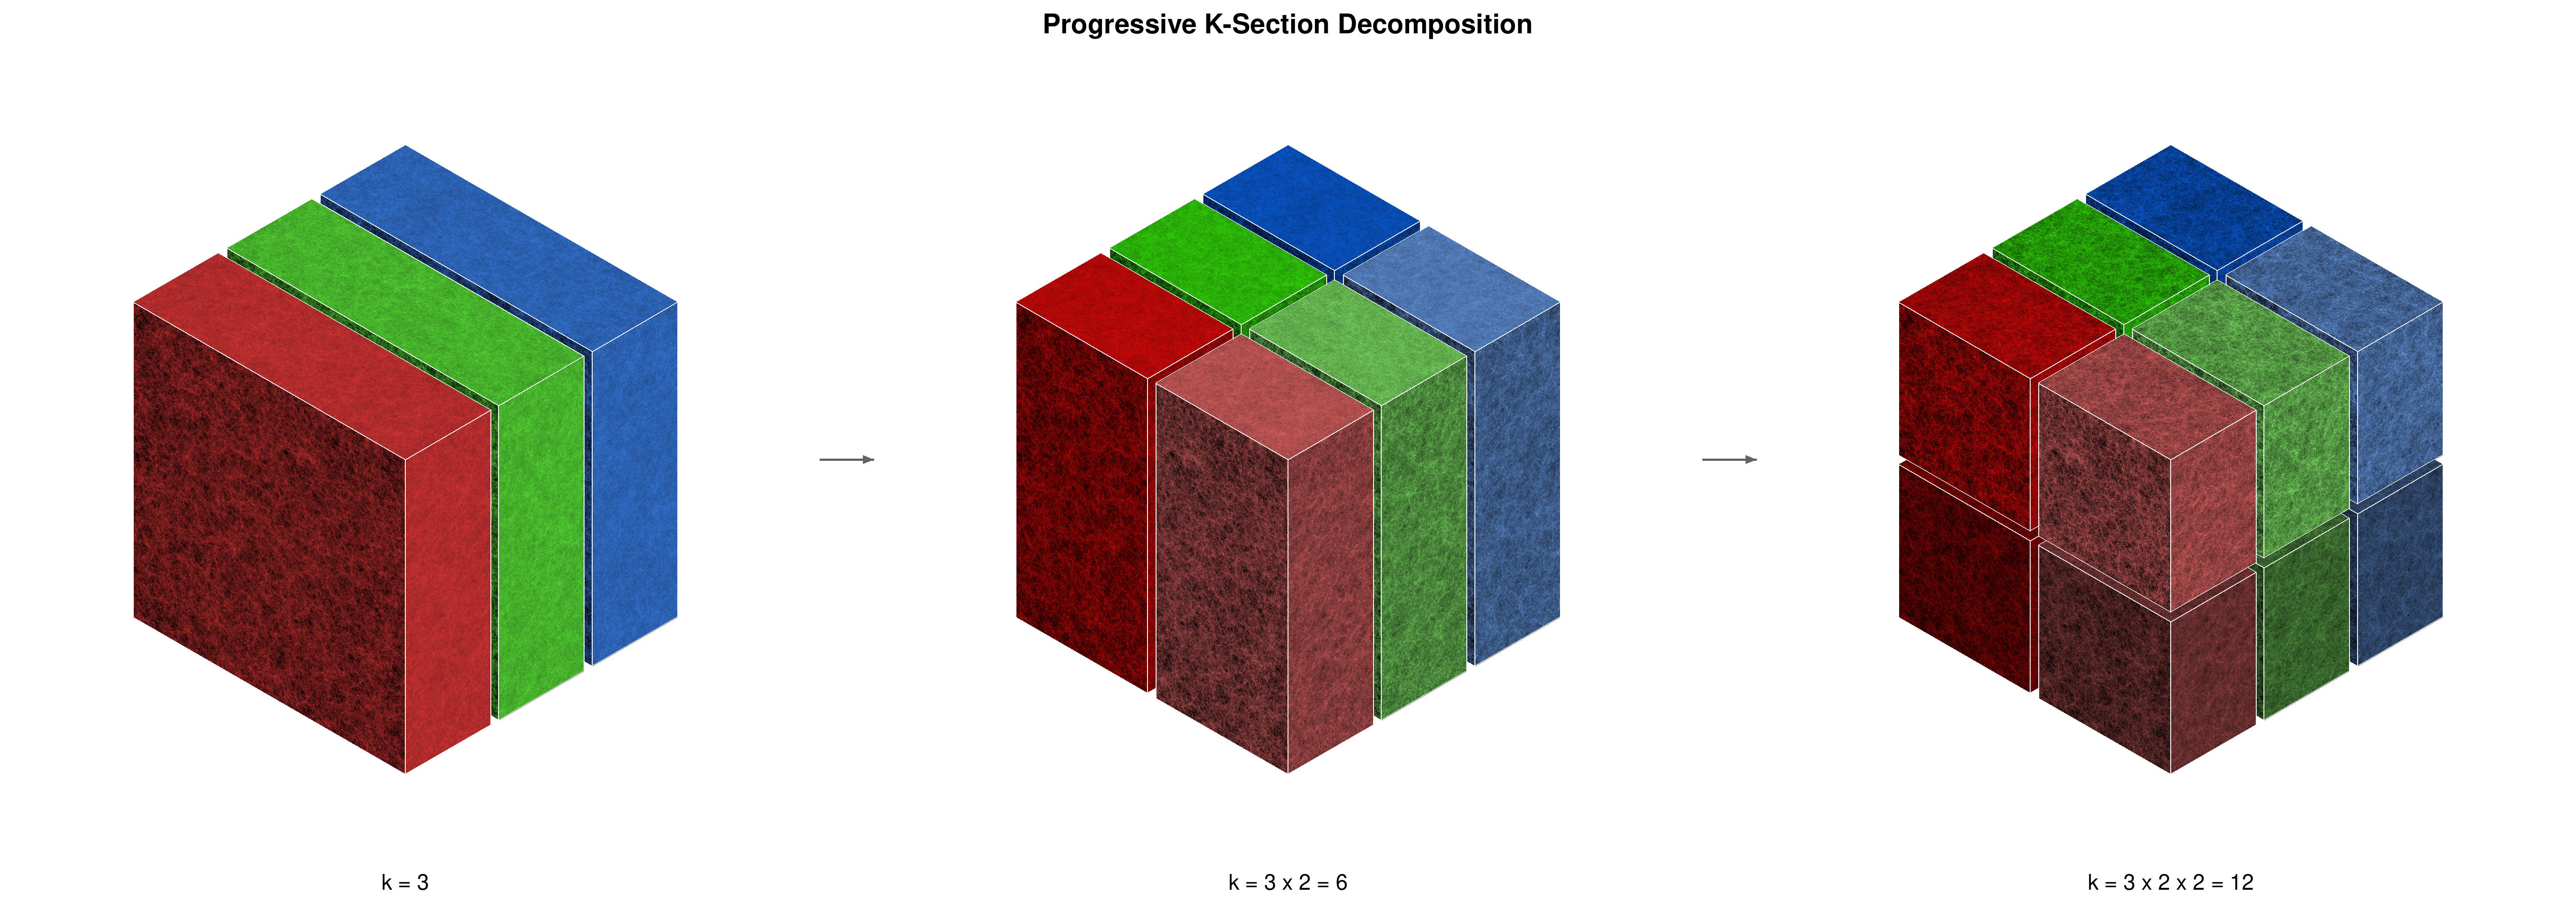
\includegraphics[width=\textwidth]{ksection_progressive.png}
\caption{Progressive k-section decomposition for $k_1 \times k_2 \times k_3 = 3 \times 2 \times 2 = 12$ CPUs with non-uniform split positions.  \textbf{Left}: first split into 3 slabs along $x$ with unequal widths.  \textbf{Center}: each slab bisected along $y$ at load-dependent positions ($3 \times 2 = 6$ subdomains).  \textbf{Right}: final bisection along $z$ ($3 \times 2 \times 2 = 12$ subdomains).  Subdomain volumes vary by ${\sim}10$--$30\%$, reflecting load-balanced wall placement.  Each face shows projected column density $\log_{10}(1+\Sigma)$ from a $4096^3$ TSC density field.}
\label{fig:ksection_progressive}
\end{figure}

\section{Hierarchical MPI Exchange}

Two exchange routines are provided in \texttt{patch/cuda/ksection.f90}:

\begin{itemize}[leftmargin=2em]
  \item \texttt{ksection\_exchange\_dp} --- exclusive exchange (each item $\to$ exactly 1 destination CPU)
  \item \texttt{ksection\_exchange\_dp\_overlap} --- overlap exchange (items routed by spatial bounding box)
\end{itemize}

\subsection{Exclusive Exchange}

Each data item has a known destination CPU. The algorithm performs level-by-level correspondent exchange through the k-section tree, using MPI tags 100--300+level.

\subsection{Overlap Exchange}

Items have spatial extent (bounding box) and may need to reach multiple CPUs. The tree walk determines all destination CPUs whose spatial domain overlaps the item's bounding box. MPI tags 400--500+level are used.

\subsection{Periodic Boundary Conditions}

The optional \texttt{periodic=.true.} parameter enables handling of items that wrap around the domain boundary $[0, \text{scale}]$. For each wrapping dimension, $2^{n_{\text{wrap}}}-1$ shifted copies are generated via bitmask subset enumeration before the tree walk.

\section{Tree Navigation}

The arrays \texttt{ksec\_cpumin/cpumax} and \texttt{ksec\_cpu\_path} (set in \texttt{build\_ksection} and at restart via \texttt{rebuild\_ksec\_cpuranges}) enable each CPU to navigate the tree efficiently.

\section{Verification}

The exchange routines are tested in \texttt{test\_ksection\_exchange} with 4 test cases:
\begin{enumerate}
  \item Exclusive point exchange
  \item Overlap point exchange
  \item Full overlap exchange
  \item Periodic overlap exchange (20\% radius items)
\end{enumerate}
All tests pass.


%======================================================
\chapter{Ghost Zone Exchange via K-Section}
%======================================================

\section{AMR Ghost Zones}

The standard RAMSES ghost zone exchange uses \texttt{MPI\_ISEND/IRECV} with all-to-all communication patterns. This was replaced with k-section tree-routed exchange for the \texttt{ordering='ksection'} mode.

\subsection{Modified File}

\texttt{patch/cuda/virtual\_boundaries.kjhan.f90}

\subsection{Subroutines}

Four k-section variants were implemented:

\begin{center}
\begin{tabular}{lll}
\toprule
\textbf{Subroutine} & \textbf{Direction} & \textbf{Data Type} \\
\midrule
\texttt{make\_virtual\_fine\_dp\_ksec} & Forward & \texttt{real(dp)} \\
\texttt{make\_virtual\_fine\_int\_ksec} & Forward & \texttt{integer} \\
\texttt{make\_virtual\_reverse\_dp\_ksec} & Reverse (+= accumulate) & \texttt{real(dp)} \\
\texttt{make\_virtual\_reverse\_int\_ksec} & Reverse (+= accumulate) & \texttt{integer} \\
\bottomrule
\end{tabular}
\end{center}

\subsection{Data Packing}

Each emission grid is packed as:
\[
\texttt{sendbuf}(1{:}\text{twotondim}+2,\; i) = \bigl[\underbrace{c_1, c_2, \ldots, c_8}_{\text{cell data}},\; \underbrace{\text{myid}}_{\text{sender}},\; \underbrace{i}_{\text{index}}\bigr]
\]

The metadata (sender ID, emission index) allows the receiver to scatter data to the correct reception grid without requiring a priori knowledge of the communication pattern.

\subsection{Dispatch}

Dispatch is automatic via:
\begin{lstlisting}[style=fortran,numbers=none]
if(ordering=='ksection') then
   call make_virtual_fine_dp_ksec(xx, ilevel)
   return
end if
\end{lstlisting}

\subsection{Bulk Exchange}

Four bulk variants exchange all columns of a 2D array (e.g., \texttt{uold}, \texttt{f}, \texttt{unew}) in a single \texttt{ksection\_exchange\_dp} call:

\begin{center}
\begin{tabular}{ll}
\toprule
\textbf{Subroutine} & \textbf{Description} \\
\midrule
\texttt{make\_virtual\_fine\_dp\_bulk} & Forward bulk exchange \\
\texttt{make\_virtual\_fine\_dp\_bulk\_ksec} & Forward bulk (ksection impl.) \\
\texttt{make\_virtual\_reverse\_dp\_bulk} & Reverse bulk exchange \\
\texttt{make\_virtual\_reverse\_dp\_bulk\_ksec} & Reverse bulk (ksection impl.) \\
\bottomrule
\end{tabular}
\end{center}

Buffer layout for \texttt{ncols} variables:
\[
\texttt{sendbuf}\bigl((v{-}1) \cdot 2^{3} + j,\;\text{idx}\bigr) = \texttt{xx}(\text{icell},\; v) \quad v=1{\ldots}\text{ncols},\; j=1{\ldots}8
\]
plus 2 metadata words (sender ID, index). This reduces MPI exchanges from $N_{\text{var}}$ per level to 1 per array.

\section{build\_comm via K-Section}

The \texttt{build\_comm} subroutine's \texttt{MPI\_ALLTOALL} + \texttt{MPI\_ISEND/IRECV} pattern was also replaced with \texttt{ksection\_exchange\_dp}.

\section{MPI\_ALLTOALL Replacements}

Additional \texttt{MPI\_ALLTOALL} calls in the following files were replaced with k-section exchange:
\begin{itemize}[leftmargin=2em]
  \item \texttt{particle\_tree.kjhan.f90}
  \item \texttt{init\_part.f90}
  \item \texttt{multigrid\_fine\_commons.f90} (in \texttt{build\_parent\_comms\_mg})
\end{itemize}

\section{Pre-Allocated Buffer Pool}

Per-level small arrays (child count, peer list, MPI requests) were converted to \texttt{save} variables to eliminate ${\sim}100$ allocations/deallocations per call. The \texttt{peer\_recv} buffer uses grow-only capacity, and the first dimension must exactly match \texttt{nprops} for MPI stride correctness.


%======================================================
\chapter{Multigrid Poisson K-Section Communication}
%======================================================

\section{Motivation}

The multigrid Poisson solver (\texttt{poisson-mg}) accounts for 29--41\% of total runtime. The original MPI communication used \texttt{MPI\_ISEND/IRECV} with all-to-all patterns across all CPUs.

\section{Implementation}

Four k-section variants were added to \texttt{patch/cuda/multigrid\_fine\_commons.f90}:

\begin{center}
\begin{tabular}{lll}
\toprule
\textbf{Subroutine} & \textbf{Direction} & \textbf{Data Type} \\
\midrule
\texttt{make\_virtual\_mg\_dp\_ksec} & Forward & \texttt{real(dp)} \\
\texttt{make\_virtual\_mg\_int\_ksec} & Forward & \texttt{integer} \\
\texttt{make\_reverse\_mg\_dp\_ksec} & Reverse (+= accumulate) & \texttt{real(dp)} \\
\texttt{make\_reverse\_mg\_int\_ksec} & Reverse (+= accumulate) & \texttt{integer} \\
\bottomrule
\end{tabular}
\end{center}

\subsection{Key Differences from AMR Exchange}

The MG communication uses different data structures from the standard AMR exchange:

\begin{center}
\begin{tabular}{lll}
\toprule
\textbf{Aspect} & \textbf{AMR} & \textbf{Multigrid} \\
\midrule
Active grids & \texttt{active(ilevel)} & \texttt{active\_mg(myid,ilevel)} \\
Reception & \texttt{reception(icpu,ilevel)} & \texttt{active\_mg(icpu,ilevel)} \\
Emission & \texttt{emission(icpu,ilevel)} & \texttt{emission\_mg(icpu,ilevel)} \\
Data arrays & \texttt{xx(igrid+iskip)} & \texttt{active\_mg\%u(icell,ivar)} \\
Indexing & Global grid index & Local offset in active\_mg \\
\bottomrule
\end{tabular}
\end{center}

\subsection{Forward Exchange}

\begin{enumerate}
  \item Pack: for each \texttt{emission\_mg(icpu)\%igrid(i)}, gather \texttt{twotondim} values from \texttt{active\_mg(myid)\%u} + metadata (sender\_id, index)
  \item Exchange via \texttt{ksection\_exchange\_dp}
  \item Scatter: use metadata to write into \texttt{active\_mg(sender)\%u(ridx + step, ivar)}
\end{enumerate}

\subsection{Reverse Exchange (Accumulation)}

\begin{enumerate}
  \item Pack: for each remote \texttt{active\_mg(icpu)\%u(i + step, ivar)} + metadata
  \item Exchange via \texttt{ksection\_exchange\_dp}
  \item Accumulate: \texttt{active\_mg(myid)\%u(emission\_mg(sender)\%igrid(ridx) + step, ivar) += recvbuf}
\end{enumerate}


%======================================================
\chapter{Morton Key Octree}
%======================================================

\section{Overview}

The \texttt{nbor} array (6 neighbor pointers per grid) was replaced with a Morton key hash table for $O(1)$ neighbor lookup. This saves $6 \times 8 \times N_{\text{gridmax}}$ bytes of memory.

\subsection{Modified Files}

\begin{itemize}[leftmargin=2em]
  \item \texttt{patch/oct\_tree/morton\_keys.f90} --- Morton key computation
  \item \texttt{patch/oct\_tree/morton\_hash.f90} --- Hash table and helper functions
  \item \texttt{patch/oct\_tree/morton\_init.f90} --- Initialization and verification
  \item \texttt{patch/oct\_tree/refine\_utils.f90} --- Hash table maintenance
  \item \texttt{patch/oct\_tree/nbors\_utils.kjhan.f90} --- Neighbor lookup functions
\end{itemize}

\section{Morton Key}

A 64-bit Morton key is computed by interleaving the 3D integer coordinates (21 bits per dimension):
\[
\text{key} = \text{interleave}\bigl(\lfloor x_g \cdot 2^{l-1} \rfloor,\; \lfloor y_g \cdot 2^{l-1} \rfloor,\; \lfloor z_g \cdot 2^{l-1} \rfloor\bigr)
\]

\section{Hash Table}

A per-level open-addressing hash table with linear probing and power-of-2 capacity maps Morton keys to grid indices. The table is maintained in \texttt{make\_grid\_coarse/fine} and \texttt{kill\_grid}, with a full rebuild after each time step.

\section{Neighbor Lookup}

Two helper functions in the \texttt{morton\_hash} module:
\begin{itemize}[leftmargin=2em]
  \item \texttt{morton\_nbor\_grid(igrid, ilevel, j)} --- returns \texttt{son(nbor(igrid,j))} equivalent
  \item \texttt{morton\_nbor\_cell(igrid, ilevel, j)} --- returns \texttt{nbor(igrid,j)} equivalent
\end{itemize}

Direction convention: $j = 1{:}{-x},\; 2{:}{+x},\; 3{:}{-y},\; 4{:}{+y},\; 5{:}{-z},\; 6{:}{+z}$.

\section{nbor Array Removal (Phase 4)}

The \texttt{nbor} array is allocated as \texttt{allocate(nbor(1:1,1:1))} (minimum size to avoid compilation errors). All code paths use Morton lookup exclusively.


%======================================================
\chapter{Memory-Based Load Balancing}
%======================================================

\section{Motivation}

Standard RAMSES load balancing distributes cells evenly across CPUs, but cells with many particles consume significantly more memory. Memory-based balancing weights each cell by its memory footprint.

\section{Cost Function}

\[
\text{cell\_cost} = \frac{\texttt{mem\_weight\_grid}}{\text{twotondim}} + \text{numbp}(\text{igrid}) \times \frac{\texttt{mem\_weight\_part}}{\text{twotondim}}
\]

where:
\begin{itemize}[leftmargin=2em]
  \item \texttt{mem\_weight\_grid} = 270 (default) --- memory per grid in dp-equivalents
  \item \texttt{mem\_weight\_part} = 12 (default) --- memory per particle in dp-equivalents
\end{itemize}

\section{Implementation Details}

\begin{itemize}[leftmargin=2em]
  \item All histogram variables use 64-bit integers (\texttt{integer(i8b)}) with \texttt{MPI\_INTEGER8}
  \item \texttt{numbp} is synchronized for virtual/reception grids before cost computation, then restored afterwards
  \item The \texttt{numbp} restore uses a save/restore pattern to avoid breaking the particle tree
\end{itemize}

\section{Parameters}

Controlled by three namelist parameters in \texttt{\&RUN\_PARAMS}:
\begin{itemize}[leftmargin=2em]
  \item \texttt{memory\_balance = .true.} --- enable memory-based balancing
  \item \texttt{mem\_weight\_grid = 270} --- grid memory weight
  \item \texttt{mem\_weight\_part = 12} --- particle memory weight
\end{itemize}


%======================================================
\chapter{Memory Savings: Large Array Optimization}
%======================================================

\section{Overview}

Several large arrays were eliminated or converted to on-demand allocation to reduce steady-state memory usage by ${\sim}960$\,MB (for \texttt{ngridmax}=5M).

\begin{center}
\begin{tabular}{llr}
\toprule
\textbf{Array} & \textbf{Strategy} & \textbf{Savings} \\
\midrule
\texttt{hilbert\_key} & \texttt{allocate(1:1)} for ksection & ${\sim}640$\,MB \\
\texttt{bisec\_ind\_cell} + \texttt{cell\_level} & On-demand alloc/dealloc & ${\sim}320$\,MB \\
\texttt{defrag\_map} & Local scratch during defrag & minor \\
\texttt{nbor} & \texttt{allocate(1:1,1:1)} (Morton) & ${\sim}240$\,MB \\
\bottomrule
\end{tabular}
\end{center}


%======================================================
\chapter{IC Reading with Stream Access}
%======================================================

\section{Motivation}

Sequential Fortran I/O requires reading all preceding planes to reach a target plane, which is $O(n^2)$ for large files. Stream access enables direct byte-offset seeks.

\section{Implementation}

Fortran 2003 \texttt{ACCESS='STREAM'} is used with computed byte offsets:

\begin{lstlisting}[style=fortran,numbers=none]
hdr_bytes = 52 + (i3-1)*plane_bytes + 5
plane_bytes = n1*n2*4 + 8  ! data + 2 record markers
\end{lstlisting}

Applied to hydro IC (deltab, velocity, temperature), particle velocity and position files. Only for \texttt{multiple=.false.} mode.

\subsection{Modified Files}
\begin{itemize}[leftmargin=2em]
  \item \texttt{patch/Horizon5-master-2/init\_flow\_fine.f90}
  \item \texttt{init\_part.f90}
\end{itemize}


%======================================================
\chapter{Load Balance Profiling and Tuning}
%======================================================

\section{Internal Timing}

Detailed timing breakdown was added to \texttt{load\_balance} in \texttt{patch/cuda/load\_balance.kjhan.f90}:

\begin{center}
\begin{tabular}{llr}
\toprule
\textbf{Section} & \textbf{Description} & \textbf{Typical (s/step)} \\
\midrule
\texttt{numbp\_sync} & MPI sync of numbp for virtual grids & 0.8--1.0 \\
\texttt{cmp\_new\_cpu\_map} & Build ksection + compute new map & 0.4--0.6 \\
\texttt{expand\_pass} & build\_comm + make\_virtual loop & 0.8--1.5 \\
\texttt{grid\_migration} & Linked-list reconnection & $< 0.01$ \\
\texttt{allreduce+cpumap\_update} & MPI\_ALLREDUCE $\times$4 + cpu\_map & 2.3--3.3 \\
\texttt{shrink\_pass} & flag\_fine + build\_comm loop & 0.4--1.0 \\
\bottomrule
\end{tabular}
\end{center}

\section{nremap Tuning}

The \texttt{nremap} parameter controls load balancing frequency (every $N$ coarse steps). Testing with 200M particles on 12 ranks showed:

\begin{center}
\begin{tabular}{rrrrl}
\toprule
\textbf{nremap} & \textbf{Total (s)} & \textbf{Loadbal (s)} & \textbf{Speedup} & \textbf{Note} \\
\midrule
1 & 303.8 & 64.4 (21.2\%) & --- & Baseline \\
3 & 269.9 & 24.7 (9.1\%) & 1.13$\times$ & \\
5 & 249.8 & 15.7 (6.3\%) & \textbf{1.22$\times$} & \textbf{Optimal} \\
10 & 258.6 & 11.6 (4.5\%) & 1.17$\times$ & Imbalance grows \\
\bottomrule
\end{tabular}
\end{center}

\begin{infobox}[Default Setting]
\texttt{nremap=5} is set as the default. All four configurations produce \textbf{bit-identical} results: \texttt{econs=3.77E-03}, \texttt{epot=-1.88E-06}, \texttt{ekin=1.23E-06} at step 10.
\end{infobox}

\section{Min/Max Memory Reporting}

The \texttt{writemem\_minmax} subroutine prints per-step min/max memory usage across all MPI ranks.


%======================================================
\chapter{Zoom-In Simulation Setup}
\label{ch:zoomin}
%======================================================

\section{Overview}

This chapter describes how to configure and run a cosmological zoom-in simulation with cuRAMSES, targeting ${\sim}1$\,kpc physical resolution within a selected sub-region of a larger cosmological volume. The setup uses:

\begin{itemize}[leftmargin=2em]
  \item \textbf{Box size}: 10\,$h^{-1}$\,Mpc (comoving)
  \item \textbf{Zoom region}: ${\sim}1.25$\,$h^{-1}$\,Mpc (centered, with padding from MUSIC)
  \item \textbf{IC levels}: 7--11 (generated by MUSIC), corresponding to base $128^3$ up to effective $2048^3$
  \item \textbf{AMR levels}: up to 14 (adaptive refinement beyond IC levels)
  \item \textbf{Physics}: hydrodynamics, gravity, radiative cooling, star formation, and AGN feedback
\end{itemize}

The main challenge in zoom-in simulations is preventing the AMR machinery from refining the entire box (which would exhaust memory). This is solved by using a passive scalar variable as a \emph{zoom geometry mask} that restricts refinement to the zoom region during initialization.


\section{Initial Conditions}

\subsection{MUSIC Configuration}

Initial conditions are generated by the MUSIC code with a multi-level zoom setup. The MUSIC configuration file specifies the base resolution, zoom region, and cosmological parameters.

\begin{codebox}[zoomin\_10Mpc.conf]
\begin{lstlisting}[style=bash,numbers=none]
[setup]
boxlength       = 10          # Box size in Mpc/h
zstart          = 50          # Starting redshift
levelmin        = 7           # Base grid: 2^7 = 128^3
levelmin_TF     = 7           # Transfer function grid
levelmax        = 11          # Zoom finest: 2^11 = 2048^3 effective
padding         = 8
overlap         = 4
ref_center      = 0.5, 0.5, 0.5
ref_extent      = 0.04, 0.04, 0.04
align_top       = yes
baryons         = yes
use_2LPT        = yes
periodic_TF     = yes

[cosmology]
# Planck 2018 (TT,TE,EE+lowE+lensing)
Omega_m         = 0.3111
Omega_L         = 0.6889
Omega_b         = 0.04
H0              = 67.66
sigma_8         = 0.8102
nspec           = 0.9665
transfer        = eisenstein

[output]
format          = grafic2
filename        = IC_zoomin
\end{lstlisting}
\end{codebox}

\subsection{Generated IC Structure}

MUSIC produces a directory hierarchy with one sub-directory per refinement level:

\begin{center}
\begin{tabular}{cccl}
\toprule
\textbf{Level} & \textbf{Grid Size} & \textbf{Resolution} & \textbf{Coverage} \\
\midrule
7 & $128^3$ & ${\sim}78$\,kpc/$h$ & Entire box \\
8 & variable & ${\sim}39$\,kpc/$h$ & Zoom region + padding \\
9 & variable & ${\sim}20$\,kpc/$h$ & Zoom region + padding \\
10 & variable & ${\sim}10$\,kpc/$h$ & Zoom region + padding \\
11 & variable & ${\sim}5$\,kpc/$h$ & Zoom region (finest IC) \\
\bottomrule
\end{tabular}
\end{center}

Each level directory contains GRAFIC2 binary files: \texttt{ic\_deltab} (baryon overdensity), \texttt{ic\_velcx/y/z} (baryon velocities), \texttt{ic\_velcdx/y/z} (dark matter velocities), \texttt{ic\_poscdx/y/z} (dark matter position offsets), and \texttt{ic\_refmap} (refinement map, level~7 only).


\section{Zoom Geometry Scalar (\texttt{ic\_pvar\_00006})}

\begin{important}
This is the single most critical aspect of the zoom-in setup. Incorrect configuration of the zoom geometry scalar will cause the entire box to be refined, leading to immediate memory exhaustion.
\end{important}

\subsection{The Problem}

In a standard RAMSES simulation, the \texttt{init\_refmap} subroutine (called when \texttt{ivar\_refine=0}) reads the \texttt{ic\_refmap} file and sets \texttt{cpu\_map2=1} for cells that should be refined. However, the default \texttt{flag\_utils} logic using \texttt{cpu\_map2} applies refinement uniformly wherever the map is set, without distinguishing between zoom and background regions at higher AMR levels. This causes the entire box to be recursively refined, rapidly exhausting memory.

\subsection{The Solution: Passive Scalar Mask}

The solution uses the 6th passive scalar variable (\texttt{ic\_pvar\_00006}) as a zoom geometry indicator. With \texttt{NVAR=11} (5~hydro + 1~metal + 5~passive), the 6th passive scalar corresponds to hydro variable index 11. Setting \texttt{ivar\_refine=11} activates a different refinement criterion in \texttt{flag\_utils}:

\begin{lstlisting}[style=fortran,numbers=none]
! In flag_utils.kjhan.f90 (during init):
if(ivar_refine > 0) then
   do i=1,ncell
      ok(i) = ok(i) .or. &
           (uold(ind_cell(i),ivar_refine) / uold(ind_cell(i),1) &
            > var_cut_refine)
   end do
end if
\end{lstlisting}

This checks whether the passive scalar (divided by density for the conserved-to-primitive conversion) exceeds \texttt{var\_cut\_refine} (typically 0.01). Cells in the zoom region have a scalar value of 1.0 and pass the test; background cells have 0.0 and are skipped.

\subsection{How It Works at Each Stage}

\begin{enumerate}
  \item \textbf{During initialization} (\texttt{init=.true.}): When \texttt{ivar\_refine} is nonzero, \texttt{init\_refmap} is \emph{not} called (line~31 of \texttt{amr/init\_refine.f90}):
\begin{lstlisting}[style=fortran,numbers=none]
if(ivar_refine==0) call init_refmap
\end{lstlisting}
  Instead, \texttt{init\_flow} loads the hydro IC (including \texttt{ic\_pvar\_00006}) and the refinement flag is set by the passive scalar criterion: $\texttt{uold}(\text{cell},11)/\texttt{uold}(\text{cell},1) > 0.01$.

  \item \textbf{After initialization} (\texttt{init=.false.}): The refinement criterion switches to the standard density-based Lagrangian criterion (\texttt{m\_refine}). The \texttt{cpu\_map2} array is set by \texttt{rho\_fine} with the \texttt{mass\_cut\_refine} parameter filtering out heavy background dark matter particles, ensuring that only the zoom region (populated by light, high-resolution particles) triggers further refinement.
\end{enumerate}

\subsection{Creating \texttt{ic\_pvar\_00006}}

The Python script \texttt{test\_ksection/create\_pvar006.py} generates the zoom geometry scalar for each IC level:

\begin{itemize}[leftmargin=2em]
  \item \textbf{Level 7} (base): Reads \texttt{ic\_refmap} from the level~7 directory. Nonzero entries (zoom cells) are set to 1.0; zero entries (background) are set to 0.0. The result is written in GRAFIC2 format as \texttt{ic\_pvar\_00006}.
  \item \textbf{Levels 8+} (zoom sub-levels): All cells are set to 1.0, since the entire grid at these levels lies within the zoom region by construction.
\end{itemize}

\begin{codebox}[create\_pvar006.py (core logic)]
\begin{lstlisting}[style=bash,numbers=none]
for level in LEVELS:
    if level == base_level:
        # Read ic_refmap, convert: nonzero -> 1.0, zero -> 0.0
        refmap = read_grafic2_data(refmap_file, n1, n2, n3)
        pvar = np.where(refmap != 0, 1.0, 0.0).astype(np.float32)
    else:
        # Zoom sub-levels: all cells = 1.0
        pvar = np.ones((n3, n2, n1), dtype=np.float32)
    write_grafic2(pvar_file, header_bytes, pvar)
\end{lstlisting}
\end{codebox}

\begin{infobox}[Editing the Script]
Before running, edit the \texttt{IC\_DIR} variable in \texttt{create\_pvar006.py} to point to your IC directory, and adjust \texttt{LEVELS} to match the levels generated by MUSIC.
\end{infobox}

\subsection{mass\_cut\_refine}

After initialization, \texttt{rho\_fine} computes the density field used to set \texttt{cpu\_map2} for refinement flagging. The \texttt{mass\_cut\_refine} parameter acts as a mass filter:

\begin{lstlisting}[style=fortran,numbers=none]
! In rho_fine.f90:
if(mass_cut_refine > 0.0) then
   do j = 1, np
      if(ttt(j) == 0d0) then          ! dark matter only
         ok(j) = ok(j) .and. mmm(j) < mass_cut_refine
      endif
   end do
endif
\end{lstlisting}

Particles heavier than \texttt{mass\_cut\_refine} are excluded from the density computation, so only high-resolution zoom particles contribute to the refinement map. Set \texttt{mass\_cut\_refine} to a value between the zoom-region DM particle mass and the next-coarser level's DM particle mass. Refer to the table in Chapter~\ref{ch:quickstart} for recommended values.


\section{Memory Considerations}

\subsection{ngridtot Sizing}

RAMSES allocates all grid-related arrays at startup based on \texttt{ngridmax} (per-CPU maximum grids). When \texttt{ngridtot} is specified, \texttt{ngridmax} is computed as \texttt{ngridtot/ncpu}. The critical constraint is:

\begin{important}
The \textbf{total virtual memory} allocated by all MPI ranks on a node must not exceed the kernel's \texttt{CommitLimit}. Exceeding this causes the OOM killer to terminate the process (SIGNAL~9).
\end{important}

\subsection{CommitLimit}

The Linux kernel's \texttt{CommitLimit} determines the maximum total virtual memory that can be allocated:
\[
\texttt{CommitLimit} = \texttt{RAM} \times \frac{\texttt{overcommit\_ratio}}{100} + \texttt{swap}
\]

Check the current value:
\begin{codebox}[Check CommitLimit]
\begin{lstlisting}[style=bash,numbers=none]
grep CommitLimit /proc/meminfo
\end{lstlisting}
\end{codebox}

On systems without swap (common for HPC nodes), \texttt{CommitLimit = RAM $\times$ overcommit\_ratio/100}. The default \texttt{overcommit\_ratio} is 50, so a 256\,GB node has ${\sim}128$\,GB CommitLimit.

\subsection{Virtual vs. Physical Memory}

RAMSES allocates the full \texttt{ngridmax}-sized arrays at startup, consuming virtual memory immediately. Physical (resident) memory grows as grids are actually created during the simulation. The key arrays that dominate virtual memory usage are:

\begin{center}
\begin{tabular}{lll}
\toprule
\textbf{Array} & \textbf{Size} & \textbf{Per-grid bytes} \\
\midrule
\texttt{uold(1:ncell,1:nvar)} & $8 \times 8 \times \text{nvar}$ & $8 \times 8 \times 11 = 704$ \\
\texttt{unew(1:ncell,1:nvar)} & same & 704 \\
\texttt{f(1:ncell,1:3)} & $8 \times 8 \times 3$ & 192 \\
\texttt{son/father/next/prev} & $8 \times 8$ each & $4 \times 64 = 256$ \\
\texttt{phi/rho} & $8 \times 8$ each & $2 \times 64 = 128$ \\
\texttt{flag1/flag2/cpu\_map/map2} & $4 \times 8$ each & $4 \times 32 = 128$ \\
\bottomrule
\end{tabular}
\end{center}

\begin{remark}[Rule of Thumb]
As a rough estimate, each grid (oct = 8 cells) requires ${\sim}2$--$3$\,kB of virtual memory across all arrays. For \texttt{ngridmax}=25\,million (i.e., \texttt{ngridtot}=200M with 8~CPUs), each rank allocates ${\sim}50$--75\,GB of virtual memory. Ensure that \texttt{ncpu $\times$ per\_rank\_virtual $<$ CommitLimit}.
\end{remark}


%======================================================
\chapter{HDF5 I/O}
\label{ch:hdf5}
%======================================================

\section{Overview}

Standard RAMSES writes one binary file per MPI process per data type (AMR, hydro, gravity, particles), producing $O(N_{\text{cpu}} \times 4)$ files per snapshot. This creates file management challenges at high core counts and requires the same number of MPI processes for restart.

The HDF5 I/O module replaces the per-CPU binary output with a single HDF5 file per snapshot, using MPI parallel I/O (collective hyperslab writes) for performance. Key benefits:

\begin{itemize}[leftmargin=2em]
  \item \textbf{Single file}: one \texttt{data\_NNNNN.h5} per snapshot instead of thousands of files
  \item \textbf{Parallel I/O}: MPI-IO backend ensures scalable write/read performance
  \item \textbf{Self-describing}: HDF5 groups and attributes contain all metadata
  \item \textbf{Cross-format}: \texttt{informat} and \texttt{outformat} can differ, enabling binary-to-HDF5 conversion
\end{itemize}

\begin{infobox}[Compilation]
HDF5 support requires compilation with \texttt{make HDF5=1}. The HDF5 library must be built with \texttt{--enable-parallel} and \texttt{--enable-fortran} for the Intel \texttt{ifx} compiler. See Section~\ref{sec:hdf5_build} for build instructions.
\end{infobox}


\section{Building HDF5}
\label{sec:hdf5_build}

The HDF5 library must be compiled from source with parallel (MPI-IO) and Fortran support matching the Intel compiler used for RAMSES.

\begin{codebox}[Build HDF5 from source]
\begin{lstlisting}[style=bash,numbers=none]
wget https://github.com/HDFGroup/hdf5/releases/download/\
  hdf5_1.14.5/hdf5-1.14.5.tar.gz
tar xf hdf5-1.14.5.tar.gz && cd hdf5-1.14.5
CC=mpiicc FC=mpiifx ./configure \
  --enable-fortran --enable-parallel \
  --prefix=$HOME/local/hdf5
make -j8 && make install
\end{lstlisting}
\end{codebox}

The key configure flags:
\begin{itemize}[leftmargin=2em]
  \item \texttt{--enable-parallel}: MPI-IO support for collective parallel reads/writes
  \item \texttt{--enable-fortran}: generates \texttt{hdf5.mod} (Fortran module) compatible with \texttt{ifx}
\end{itemize}

Then build RAMSES with the \texttt{HDF5=1} flag:

\begin{codebox}[Build RAMSES with HDF5]
\begin{lstlisting}[style=bash,numbers=none]
cd bin
make clean
make HDF5=1
\end{lstlisting}
\end{codebox}

The Makefile conditionally adds:
\begin{lstlisting}[style=fortran,numbers=none]
HDF5_DIR = $(HOME)/local/hdf5
FFLAGS += -DHDF5 -I$(HDF5_DIR)/include
LIBS += -L$(HDF5_DIR)/lib -lhdf5_fortran -lhdf5 -lz \
        -Wl,-rpath,$(HDF5_DIR)/lib
\end{lstlisting}

Without \texttt{HDF5=1}, the code compiles identically to before (all HDF5 code is guarded by \texttt{\#ifdef HDF5}).


\section{Namelist Parameters}

Two parameters in \texttt{\&OUTPUT\_PARAMS} control the I/O format:

\begin{center}
\begin{tabular}{llll}
\toprule
\textbf{Parameter} & \textbf{Type} & \textbf{Default} & \textbf{Description} \\
\midrule
\texttt{outformat} & char(10) & \texttt{'original'} & Output format: \texttt{'original'} or \texttt{'hdf5'} \\
\texttt{informat} & char(10) & \texttt{'original'} & Restart format: \texttt{'original'} or \texttt{'hdf5'} \\
\bottomrule
\end{tabular}
\end{center}

\begin{codebox}[Example namelist]
\begin{lstlisting}[style=fortran,numbers=none]
&OUTPUT_PARAMS
noutput=1
aout=1.0
foutput=5
outformat='hdf5'    ! write HDF5 snapshots
/
\end{lstlisting}
\end{codebox}

For restart from an HDF5 checkpoint:
\begin{codebox}[Restart from HDF5]
\begin{lstlisting}[style=fortran,numbers=none]
&RUN_PARAMS
nrestart=1
/
&OUTPUT_PARAMS
informat='hdf5'     ! read HDF5 checkpoint
outformat='hdf5'    ! continue writing HDF5
/
\end{lstlisting}
\end{codebox}


\section{HDF5 File Structure}

Each snapshot produces a single file \texttt{output\_NNNNN/data\_NNNNN.h5} with the following group hierarchy:

\begin{lstlisting}[style=bash,numbers=none]
data_NNNNN.h5
  /header/              (attrs: ncpu, ndim, nlevelmax, nstep,
                         boxlen, time, aexp, H0, omega_m, ...)
      tout[noutput]     (dataset)
      aout[noutput]     (dataset)
      dtold[nlevelmax]  (dataset)
      dtnew[nlevelmax]  (dataset)
  /domain/              (ksection tree or bound_key)
  /coarse/
      son[ncoarse]      (dataset: integer)
      cpu_map[ncoarse]  (dataset: integer)
  /amr/level_LL/
      xg[ngrid_total x 3]           (grid centres)
      son[ngrid_total x twotondim]   (son indices)
      cpu_map[ngrid_total x twotondim]
      nbor[ngrid_total x twondim]    (Morton-computed)
      ngrid_per_cpu[ncpu]
  /hydro/level_LL/
      uold[ngrid_total x twotondim x nvar]
  /gravity/level_LL/
      phi[ngrid_total x twotondim]
      f[ngrid_total x twotondim x ndim]
  /particles/
      x[npart_total x ndim]    (positions)
      v[npart_total x ndim]    (velocities)
      m[npart_total]            (masses)
      id[npart_total]           (particle IDs)
      level[npart_total]        (AMR level)
      tp[npart_total]           (birth time)
      zp[npart_total]           (metallicity)
      npart_per_cpu[ncpu]
  /sinks/
      idsink, msink, xsink, vsink, tsink, ...
\end{lstlisting}

\subsection{Parallel Write Strategy}

Each AMR level is written using collective MPI-IO hyperslabs:

\begin{enumerate}
  \item \texttt{MPI\_Allgather(ngrid\_local)} to compute per-CPU offsets
  \item Each CPU writes its portion via an HDF5 hyperslab selection
  \item Collective I/O ensures efficient parallel access to the shared file
\end{enumerate}

Particles use the same hyperslab pattern: \texttt{MPI\_Allgather(npart\_local)} for offsets, then collective write.


\section{Implementation Files}

\begin{center}
\begin{tabular}{ll}
\toprule
\textbf{File} & \textbf{Description} \\
\midrule
\texttt{patch/cuda/ramses\_hdf5\_io.f90} & HDF5 wrapper module (create, open, write, read helpers) \\
\texttt{patch/cuda/backup\_hdf5.f90} & HDF5 output: \texttt{dump\_all\_hdf5()} \\
\texttt{patch/cuda/restore\_hdf5.f90} & HDF5 restart: \texttt{restore\_amr\_hdf5()}, etc. \\
\bottomrule
\end{tabular}
\end{center}

\subsection{Dispatch}

The HDF5 output is dispatched from \texttt{dump\_all} in \texttt{output\_amr.kjhan.f90}:

\begin{lstlisting}[style=fortran,numbers=none]
#ifdef HDF5
if(outformat == 'hdf5') then
   call dump_all_hdf5(filedir, nchar)
   goto 998  ! skip binary output
end if
#endif
\end{lstlisting}

For restart, each \texttt{init\_*} subroutine checks \texttt{informat}:

\begin{lstlisting}[style=fortran,numbers=none]
#ifdef HDF5
if(informat == 'hdf5') then
   call restore_amr_hdf5()
   return
end if
#endif
\end{lstlisting}


\section{Verification}

The HDF5 output was tested with a 5-step cosmological simulation (12~MPI ranks, levelmin=8, levelmax=10, 200M particles):

\begin{center}
\begin{tabular}{lr}
\toprule
\textbf{Metric} & \textbf{Value} \\
\midrule
Output file & \texttt{data\_00001.h5} (3.65~GB) \\
Step count & 5 \\
econs at step 5 & 4.85E-03 \\
I/O time & 4.1\,s (16.1\% of total) \\
Total runtime & 20.6\,s \\
\bottomrule
\end{tabular}
\end{center}


\section{Variable-NCPU Restart: Distributed Grid Creation}
\label{sec:varcpu-dist}

When restarting an HDF5 checkpoint with a different number of MPI ranks (\texttt{ncpu\_file} $\neq$ \texttt{ncpu}), the original implementation allocated \emph{all} grids from the file on \emph{every} rank.  For a file with 11.17\,M grids, this required \texttt{ngridmax} $\geq$ 11.17\,M per rank, consuming $\sim$20\,GB per rank.  With 32 ranks the total memory exceeded 640\,GB, causing out-of-memory failures on systems with $\leq$560\,GB.

\subsection{Distributed Algorithm}

The new implementation creates only the grids each rank actually needs.  For each level $L = 1$ to \texttt{nlevelmax\_file}:

\begin{enumerate}
  \item \textbf{Phase 1 --- Active grid creation.}
    All ranks read the file data for level~$L$ (grid positions and \texttt{son\_flag}), but each rank only allocates grids whose father cell satisfies \texttt{cpu\_map(father\_cell) == myid}.
    For $L \geq 2$, the father grid is located via Morton hash lookup at level $L-1$; if the lookup returns zero (father not present on this rank), the grid is not local and is skipped.
    Active grids have their \texttt{xg}, \texttt{flag1}, \texttt{cpu\_map}, \texttt{cpu\_map2}, \texttt{father}, and \texttt{son} set from the file data, and are inserted into the Morton hash table.

  \item \textbf{Phase 2 --- Virtual grid creation.}
    Virtual (ghost) grids are created using RAMSES's existing refinement infrastructure:
    \begin{itemize}
      \item $L = 1$: \texttt{flag\_coarse} $\to$ \texttt{refine\_coarse}
      \item $L \geq 2$: \texttt{refine\_fine($L-1$)}
    \end{itemize}
    Since active grids already set \texttt{son(father\_cell)} $> 0$, \texttt{refine\_fine} skips those cells and only creates virtual grids where \texttt{flag1 == 1} and \texttt{son == 0}.
    The flag \texttt{balance = .true.}\ causes \texttt{make\_grid\_fine} to skip hydro variable interpolation (line~791 of \texttt{refine\_utils.f90}).

  \item \textbf{Communication setup.}
    \texttt{build\_comm($L$)} establishes emission/reception arrays, followed by
    \texttt{make\_virtual\_fine\_int} exchanges for \texttt{flag1}, \texttt{cpu\_map}, and \texttt{cpu\_map2}.
    This ensures the next level's \texttt{refine\_fine} has correct flag values on virtual grids.
\end{enumerate}

After all levels, hydro and Poisson data are restored from the file (same read-all-scatter pattern) and exchanged to virtual grids via \texttt{make\_virtual\_fine\_dp}.

\subsection{Key Design Decisions}

\begin{itemize}
  \item \textbf{Father lookup as filter.}
    For $L \geq 2$, the Morton hash lookup at level $L-1$ serves as an implicit ownership test: if the father grid does not exist locally, the child grid cannot be active on this rank.
  \item \textbf{Hash table sizing.}
    The per-level hash table is sized for local grids: \texttt{max(4 * (ngrid\_total / ncpu + 1), 16)} instead of \texttt{2 * ngrid\_total}, reducing hash table memory proportionally.
  \item \textbf{No changes to other files.}
    \texttt{refine\_coarse}, \texttt{refine\_fine}, \texttt{build\_comm}, \texttt{authorize\_fine}, and \texttt{make\_grid\_fine} all work unmodified.
    The same-ncpu restart path is also unchanged.
\end{itemize}

\subsection{Verification}

A 12-CPU HDF5 checkpoint (levelmin=8, levelmax=10, 200M particles) was restarted with 8~CPUs.  The reference is the same checkpoint restarted with 12~CPUs (same-ncpu path).

\begin{center}
\begin{tabular}{lrr}
\toprule
\textbf{Metric} & \textbf{Reference (12$\to$12)} & \textbf{Distributed (12$\to$8)} \\
\midrule
ngrid per rank       & 2,396,745    & 352,379   \\
Memory per rank      & 8.0\,GB      & 6.9\,GB   \\
Grid reduction       & ---          & 6.8$\times$ \\
\bottomrule
\end{tabular}
\end{center}

\begin{center}
\begin{tabular}{lrrrrrr}
\toprule
\textbf{Step} & \multicolumn{2}{c}{\textbf{econs}} & \multicolumn{2}{c}{\textbf{epot}} & \multicolumn{2}{c}{\textbf{ekin}} \\
 & Ref & Dist & Ref & Dist & Ref & Dist \\
\midrule
6  & 8.18E-03 & 8.17E-03 & $-$1.01E-06 & $-$1.01E-06 & 6.49E-07 & 6.49E-07 \\
7  & 7.26E-03 & 7.25E-03 & $-$1.26E-06 & $-$1.26E-06 & 8.17E-07 & 8.17E-07 \\
8  & 6.43E-03 & 6.42E-03 & $-$1.48E-06 & $-$1.48E-06 & 9.63E-07 & 9.63E-07 \\
9  & 5.79E-03 & 5.79E-03 & $-$1.68E-06 & $-$1.68E-06 & 1.09E-06 & 1.09E-06 \\
10 & 5.26E-03 & 5.25E-03 & $-$1.88E-06 & $-$1.88E-06 & 1.23E-06 & 1.23E-06 \\
\bottomrule
\end{tabular}
\end{center}

The epot and ekin values are \textbf{identical} across all steps.  The econs differences (last display digit) arise from different domain decomposition with 8 vs.\ 12 CPUs.  With 32~CPUs the grid reduction would be $\sim$20$\times$, bringing the previously OOM scenario (640\,GB) well within a 560\,GB memory budget.


\section{Poisson MG Fine-Level Optimization}

The multigrid Poisson solver (\texttt{poisson-mg}) is typically the single largest time consumer, accounting for 29--55\% of total runtime. Several optimizations were applied to the fine-level V-cycle in \texttt{poisson/multigrid\_fine\_fine.kjhan.f90}:

\subsection{Precomputed Neighbor Grid Array}

Before entering the V-cycle iteration loop, all 6-directional neighbor grids are precomputed and stored in a contiguous array:

\begin{lstlisting}[style=fortran,numbers=none]
! nbor_grid_fine(0:twondim, 1:ngrid)
!   index 0 = self (igrid_amr)
!   index 1..6 = neighbor grids in -x,+x,-y,+y,-z,+z
call precompute_nbor_grid_fine(ilevel)
\end{lstlisting}

This replaces per-cell \texttt{morton\_nbor\_grid} calls inside the Gauss-Seidel and residual loops with simple array lookups, eliminating hash table probes from the innermost loops.

\subsection{Merged Red-Black Gauss-Seidel Exchange}

The standard multigrid implementation performs a ghost zone exchange after each half-sweep of the red-black Gauss-Seidel smoother:
\begin{center}
\texttt{red} $\to$ \texttt{exchange} $\to$ \texttt{black} $\to$ \texttt{exchange}
\end{center}

This was simplified to:
\begin{center}
\texttt{red} $\to$ \texttt{black} $\to$ \texttt{exchange}
\end{center}

The black sweep uses slightly stale ghost values from the red sweep (``chaotic relaxation''), which does not affect multigrid convergence. This reduces the number of MPI exchanges per iteration from 9 to 5 (a 44\% reduction in communication calls).

\subsection{Residual and Norm Single Pass}

The residual computation and the $L^2$ norm reduction were fused into a single pass:

\begin{lstlisting}[style=fortran,numbers=none]
! Optional norm2 argument: if present, compute
! both residual and L2 norm in one sweep
call cmp_residual_mg_fine(ilevel, norm2)
\end{lstlisting}

This eliminates a redundant loop over all cells when both the residual and its norm are needed (at the first iteration and after post-smoothing).

\subsection{Division to Multiplication}

In the Gauss-Seidel fast path, the division by \texttt{dtwondim} was replaced with multiplication by a precomputed reciprocal:

\begin{lstlisting}[style=fortran,numbers=none]
real(dp) :: oneoverdtwondim
oneoverdtwondim = 1.0d0 / dble(twondim)
! In loop:
phi = sum_neighbors * oneoverdtwondim   ! was: / dtwondim
\end{lstlisting}

\subsection{Performance Impact}

These optimizations combined reduce the Poisson solver's share of total runtime:

\begin{center}
\begin{tabular}{lr}
\toprule
\textbf{Metric} & \textbf{Value} \\
\midrule
Before optimization & 55.1\% of runtime \\
After optimization & 38.6\% of runtime \\
MPI exchange reduction & 44\% fewer calls \\
Iteration count & unchanged (Level~8: 5, Level~9: 4) \\
Convergence & verified (econs = 3.79E-03 at step~10) \\
\bottomrule
\end{tabular}
\end{center}

\begin{infobox}[Chaotic Relaxation]
The merged red-black exchange introduces a minor change in the energy conservation value (3.77E-03 $\to$ 3.79E-03) due to the slightly different relaxation path. This is well within the multigrid tolerance and does not affect physical results. The membal and nomembal tests produce identical values.
\end{infobox}


%======================================================
\chapter{Scaling Performance}
\label{ch:scaling}
%======================================================

Strong scaling tests were performed using a $200 \times 10^6$ particle cosmological simulation (levelmin=8, levelmax=10), restarted from an HDF5 checkpoint at coarse step~5 and evolved to step~10 (5 coarse steps). The test platform is a dual-socket AMD EPYC 7543 node (64 physical cores, 128 threads via SMT) with 1~TB of DDR4 memory. The code was compiled with Intel MPI (\texttt{mpiifx}) and OpenMP (\texttt{-qopenmp}).

The variable-\texttt{ncpu} restart allows the 12-rank checkpoint to be read with any number of MPI ranks. A forced \texttt{load\_balance} on the first coarse step ensures optimal grid distribution.

\section{Pure MPI Scaling}

All runs use \texttt{OMP\_NUM\_THREADS=1}.  Speedup is relative to the 2-rank baseline.

\begin{center}
\begin{tabular}{rrrrrrrrrr}
\toprule
\textbf{Ranks} & \textbf{Elapsed} & \textbf{Speedup} & \textbf{Coarse} & \textbf{Particle} & \textbf{Poisson} & \textbf{MG} & \textbf{Hydro-GZ} & \textbf{Godunov} & \textbf{LoadBal} \\
 & (s) & & (s) & (s) & (s) & (s) & (s) & (s) & (s) \\
\midrule
2   & 193.0 & 1.00$\times$ & 2.27 & 20.92 & 18.22 & 102.69 & 0.52 & 46.67 & 9.14 \\
4   & 154.8 & 1.25$\times$ & 2.59 & 16.74 & 14.76 & 82.00  & 0.89 & 36.64 & 7.62 \\
8   &  88.9 & 2.17$\times$ & 2.12 &  8.93 &  8.18 & 43.46  & 1.09 & 21.68 & 4.90 \\
16  &  58.2 & 3.31$\times$ & 2.56 &  4.67 &  4.97 & 23.90  & 1.26 & 15.88 & 3.96 \\
32  &  34.7 & 5.57$\times$ & 2.04 &  2.27 &  2.73 & 12.59  & 1.11 &  8.71 & 2.27 \\
64  &  25.9 & 7.45$\times$ & 1.91 &  1.18 &  1.64 &  7.95  & 1.13 &  5.14 & 1.61 \\
\bottomrule
\end{tabular}
\end{center}

\section{Hybrid MPI + OpenMP Scaling}

All configurations use a fixed total of 64 physical cores.  Speedup is relative to the 2-rank pure MPI baseline (193.0\,s).

\begin{center}
\begin{tabular}{rrrrrrrrrr}
\toprule
\textbf{Ranks$\times$Thr} & \textbf{Elapsed} & \textbf{Speedup} & \textbf{Coarse} & \textbf{Particle} & \textbf{Poisson} & \textbf{MG} & \textbf{Hydro-GZ} & \textbf{Godunov} & \textbf{LoadBal} \\
 & (s) & & (s) & (s) & (s) & (s) & (s) & (s) & (s) \\
\midrule
64$\times$1  & 25.9 & 7.45$\times$ & 1.91 & 1.18 & 1.64 & 7.95  & 1.13 & 5.14 & 1.61 \\
\textbf{32$\times$2}  & \textbf{22.2} & \textbf{8.71$\times$} & 1.55 & 1.37 & 1.64 & 7.23  & 0.82 & 5.19 & 1.63 \\
16$\times$4  & 24.9 & 7.76$\times$ & 1.49 & 2.23 & 2.31 & 8.81  & 0.66 & 5.22 & 2.46 \\
8$\times$8   & 30.2 & 6.40$\times$ & 1.26 & 3.80 & 3.34 & 11.35 & 0.68 & 5.46 & 3.06 \\
4$\times$16  & 44.4 & 4.34$\times$ & 1.35 & 6.99 & 5.66 & 17.22 & 0.67 & 6.21 & 5.27 \\
\bottomrule
\end{tabular}
\end{center}

\section{Key Observations}

\begin{itemize}
\item \textbf{Optimal configuration} is 32 ranks $\times$ 2 threads (22.2\,s), which is 14\% faster than 64 pure MPI ranks (25.9\,s) and $8.7\times$ faster than the 2-rank baseline.

\item \textbf{Multigrid Poisson solver (MG)} dominates runtime and scales well: 102.7\,s (2 ranks) $\to$ 7.2\,s (32$\times$2), a $14.2\times$ speedup.

\item \textbf{Godunov hydro solver} scales effectively with both MPI and OpenMP: 46.7\,s (2 ranks) $\to$ 5.2\,s (32$\times$2), a $9.0\times$ speedup.

\item \textbf{Ghost-zone exchange (Hydro-GZ)} increases slightly with MPI rank count (0.52\,s at 2 ranks $\to$ 1.13\,s at 64 ranks) due to more MPI messages, but \emph{decreases} in hybrid mode (0.82\,s at 32$\times$2) since fewer ranks means fewer messages.

\item \textbf{Hybrid advantage}: 32$\times$2 beats 64$\times$1 because halving the MPI rank count reduces communication overhead (ghost zones, load balancing) while the 2 OpenMP threads provide sufficient intra-rank parallelism for compute-bound kernels.

\item \textbf{Diminishing returns from OpenMP}: beyond 4 threads per rank, OpenMP thread synchronization overhead outweighs the communication savings, causing performance to degrade (4$\times$16: 44.4\,s, worse than 8$\times$1: 88.9\,s with only 8 total cores).

\item \textbf{Load balancing} scales well: 9.1\,s at 2 ranks $\to$ 1.6\,s at 64 ranks.  This is a per-\texttt{nremap} cost (default \texttt{nremap=5}).

\item \textbf{Physics correctness}: all configurations produce identical $e_{\rm pot} = -1.88 \times 10^{-6}$ and $e_{\rm kin} = 1.23 \times 10^{-6}$ at step~10.
\end{itemize}

\begin{infobox}[Recommended Configuration]
For a single dual-socket AMD EPYC node with 64 cores, we recommend \textbf{32 MPI ranks $\times$ 2 OpenMP threads} for cuRAMSES cosmological simulations with $\sim$$200 \times 10^6$ particles.  Set \texttt{OMP\_NUM\_THREADS=2}, \texttt{OMP\_PROC\_BIND=close}, \texttt{OMP\_PLACES=cores}, and \texttt{I\_MPI\_PIN\_DOMAIN=omp} in the job script.
\end{infobox}

\section{Per-Routine Scaling Analysis}

Table~\ref{tab:routine-mpi} shows the complete timer breakdown for pure MPI scaling, and Table~\ref{tab:routine-hybrid} for the hybrid configurations.  All times are averages across ranks in seconds.

\begin{table}[htbp]
\caption{Full timer breakdown --- pure MPI (\texttt{OMP\_NUM\_THREADS=1}).}
\label{tab:routine-mpi}
\begin{center}
\small
\begin{tabular}{lrrrrrrl}
\toprule
\textbf{Routine} & \textbf{2r} & \textbf{4r} & \textbf{8r} & \textbf{16r} & \textbf{32r} & \textbf{64r} & \textbf{Scale} \\
\midrule
poisson-mg     & 102.69 & 82.00 & 43.46 & 23.90 & 12.59 &  7.95 & 12.9$\times$ \\
godunov        &  46.67 & 36.64 & 21.68 & 15.88 &  8.71 &  5.14 &  9.1$\times$ \\
particles      &  20.92 & 16.74 &  8.93 &  4.67 &  2.27 &  1.18 & 17.7$\times$ \\
poisson        &  18.22 & 14.76 &  8.18 &  4.97 &  2.73 &  1.64 & 11.1$\times$ \\
flag           &  11.35 &  8.23 &  4.41 &  2.78 &  1.28 &  0.77 & 14.7$\times$ \\
loadbalance    &   9.14 &  7.62 &  4.90 &  3.96 &  2.27 &  1.61 &  5.7$\times$ \\
io             &   3.14 &  1.96 &  1.86 &  2.72 &  4.23 &  6.17 &  0.5$\times\downarrow$ \\
coarse levels  &   2.27 &  2.59 &  2.12 &  2.56 &  2.04 &  1.91 &  1.2$\times$ \\
courant        &   2.23 &  1.49 &  0.76 &  0.41 &  0.23 &  0.12 & 18.6$\times$ \\
hydro-gz       &   0.52 &  0.89 &  1.09 &  1.26 &  1.11 &  1.13 &  0.5$\times\downarrow$ \\
rev-gz         &   0.53 &  1.79 &  2.42 &  1.75 &  0.78 &  0.71 &  0.7$\times\downarrow$ \\
set unew       &   0.28 &  0.26 &  0.22 &  0.23 &  0.15 &  0.10 &  2.8$\times$ \\
set uold       &   1.11 &  0.77 &  0.38 &  0.24 &  0.15 &  0.10 & 11.1$\times$ \\
refine         &   0.61 &  0.86 &  0.69 &  0.62 &  0.43 &  0.27 &  2.3$\times$ \\
\midrule
\textbf{TOTAL} & 219.7  & 176.6 & 101.1 &  66.0 &  39.0 &  28.8 &  7.6$\times$ \\
\bottomrule
\end{tabular}
\end{center}
\end{table}

\begin{table}[htbp]
\caption{Full timer breakdown --- hybrid MPI+OpenMP (fixed 64 cores).}
\label{tab:routine-hybrid}
\begin{center}
\small
\begin{tabular}{lrrrrr}
\toprule
\textbf{Routine} & \textbf{64$\times$1} & \textbf{32$\times$2} & \textbf{16$\times$4} & \textbf{8$\times$8} & \textbf{4$\times$16} \\
\midrule
poisson-mg     &  7.95 &  7.23 &  8.81 & 11.35 & 17.22 \\
godunov        &  5.14 &  5.19 &  5.22 &  5.46 &  6.21 \\
particles      &  1.18 &  1.37 &  2.23 &  3.80 &  6.99 \\
poisson        &  1.64 &  1.64 &  2.31 &  3.34 &  5.66 \\
io             &  6.17 &  3.37 &  2.25 &  2.02 &  1.89 \\
loadbalance    &  1.61 &  1.63 &  2.46 &  3.06 &  5.27 \\
flag           &  0.77 &  0.89 &  1.50 &  2.47 &  4.71 \\
hydro-gz       &  1.13 &  0.82 &  0.66 &  0.68 &  0.67 \\
rev-gz         &  0.71 &  0.57 &  0.83 &  0.56 &  0.58 \\
coarse levels  &  1.91 &  1.55 &  1.49 &  1.26 &  1.35 \\
courant        &  0.12 &  0.13 &  0.13 &  0.13 &  0.14 \\
set uold       &  0.10 &  0.10 &  0.10 &  0.11 &  0.14 \\
set unew       &  0.10 &  0.10 &  0.09 &  0.09 &  0.10 \\
refine         &  0.27 &  0.28 &  0.31 &  0.25 &  0.40 \\
\midrule
\textbf{TOTAL} &  28.8 &  24.9 &  28.4 &  34.6 &  51.3 \\
\bottomrule
\end{tabular}
\end{center}
\end{table}

\subsection{Scaling Categories}

The routines fall into three distinct categories by their scaling behavior:

\begin{enumerate}
\item \textbf{Compute-bound (excellent MPI scaling).}
  \texttt{courant} (18.6$\times$), \texttt{particles} (17.7$\times$), \texttt{flag} (14.7$\times$), \texttt{poisson-mg} (12.9$\times$), \texttt{poisson} (11.1$\times$), \texttt{godunov} (9.1$\times$).
  These routines perform per-cell or per-particle work and scale nearly linearly with MPI rank count.  In the hybrid regime, they are insensitive to the MPI/OMP ratio as long as total cores $\geq 32$.

\item \textbf{Communication-bound (anti-scaling).}
  \texttt{hydro-gz} (ghost zone exchange) grows from 0.52\,s to 1.13\,s as ranks increase from 2 to 64, because more ranks means more boundary surfaces and MPI messages.  In the hybrid regime, reducing ranks to 32 or fewer recovers some of this cost ($0.82$\,s at 32$\times$2, $0.67$\,s at 4$\times$16).
  \texttt{io} (HDF5 output) degrades from 3.14\,s at 2 ranks to 6.17\,s at 64 ranks due to MPI collective I/O contention.  This is the clearest anti-scaling component: halving the rank count from 64 to 32 nearly halves the I/O time (6.17\,s $\to$ 3.37\,s).

\item \textbf{Flat (Amdahl-limited).}
  \texttt{coarse levels} remains at $\sim$2\,s regardless of configuration --- this work is inherently serial or involves global communication at the coarsest level.  It becomes a larger fraction of runtime as other components scale (from 1\% at 2 ranks to 6.6\% at 64 ranks).
\end{enumerate}

\subsection{Bottleneck Shift}

As the rank count increases, the dominant bottleneck shifts:
\begin{itemize}[nosep]
\item At 2 ranks: \texttt{poisson-mg} (46.7\%), \texttt{godunov} (21.2\%), \texttt{particles} (9.5\%)
\item At 32$\times$2: \texttt{poisson-mg} (29.1\%), \texttt{godunov} (20.9\%), \texttt{io} (13.6\%)
\item At 64$\times$1: \texttt{poisson-mg} (27.6\%), \texttt{io} (21.4\%), \texttt{godunov} (17.8\%)
\end{itemize}
At high rank counts, I/O emerges as the second-largest cost, suggesting that asynchronous or node-local I/O strategies would yield further speedup.


%======================================================
\chapter{GPU Hydro Acceleration}
\label{ch:gpu}
%======================================================

cuRAMSES supports GPU acceleration for the main hydro solver routines via CUDA.  The implementation uses a \textbf{dynamic hybrid CPU/GPU dispatch} model where OpenMP threads compete for a shared pool of GPU streams: threads that acquire a stream offload their work to the GPU, while the remaining threads continue on the CPU.  This design naturally adapts to any ratio of CPU cores to GPU streams.

\section{Architecture Overview}

The GPU acceleration is enabled at build time with \texttt{make HDF5=1 USE\_CUDA=1}.  At runtime, each MPI rank initializes a pool of 8 CUDA streams, distributed across available GPUs by local rank (\texttt{local\_rank \% device\_count}).  The multi-architecture binary supports sm\_80 (A100), sm\_86 (A10), sm\_89 (RTX 5000 Ada), and sm\_90 (H100) targets simultaneously.

\begin{infobox}[Key Files]
\begin{itemize}[nosep,leftmargin=1.5em]
\item \texttt{cuda\_stream\_pool.\{h,cu\}} --- Thread-safe stream pool with atomic acquire/release
\item \texttt{hydro\_cuda\_kernels.cu} --- CUDA kernels: \texttt{ctoprim}, \texttt{uslope}, \texttt{trace3d}, \texttt{flux}, \texttt{difmag}, \texttt{synchro}, \texttt{cmpdt}, \texttt{gradient\_phi}, \texttt{upload\_fine}
\item \texttt{hydro\_cuda\_interface.f90} --- Fortran ISO\_C\_BINDING wrappers with assumed-size \texttt{buf(*)} for safe \texttt{c\_loc} usage
\item \texttt{cuda\_commons.f90} --- Fortran module exposing stream pool to the AMR code
\end{itemize}
\end{infobox}

\section{Hybrid CPU/GPU Dispatch}

The dispatch model is illustrated for the Godunov solver (\texttt{godunov\_fine.kjhan.f90}), which accounts for $\sim$30\% of total runtime:

\begin{lstlisting}[language=Fortran,basicstyle=\small\ttfamily,frame=single,caption={Dynamic hybrid dispatch pattern},label=lst:hybrid]
!$omp parallel
  stream_slot = cuda_acquire_stream()  ! atomic, -1 if busy
  !$omp do schedule(dynamic)
  do igrid = 1, ncache, nvector
     if (stream_slot >= 0) then
        ! GPU: gather into superbatch buffer
        ! Flush when buffer full -> async GPU kernel
     else
        ! CPU: standard godfine1 computation
     end if
  end do
  !$omp end do nowait
  ! GPU thread: flush remaining buffer, release stream
!$omp end parallel
\end{lstlisting}

The \texttt{schedule(dynamic)} clause ensures load balancing: if one thread is waiting for GPU synchronization, other threads pick up the remaining iterations on CPU.  This is particularly effective when the number of OMP threads exceeds the number of GPU streams.

\subsection{Superbatch Buffering}

GPU kernel launches have significant latency ($\sim$10--50\,$\mu$s).  To amortize this, each GPU thread accumulates grid data into a \textbf{superbatch buffer} of size \texttt{SUPER\_SIZE} (typically 4096 grids) before launching a single kernel covering all accumulated grids.  The buffer is flushed when it approaches capacity or when the \texttt{omp do} loop completes.

For the Godunov solver, the superbatch contains the full stencil data (conservative variables and gravitational acceleration on a $6 \times 6 \times 6$ grid per AMR oct), and the GPU pipeline executes 5 kernels in sequence: \texttt{ctoprim} $\to$ \texttt{uslope} $\to$ \texttt{trace3d} $\to$ \texttt{flux} $\to$ \texttt{difmag}.

\subsection{Accelerated Routines}

Six routines use the hybrid dispatch pattern:

\begin{center}
\begin{tabular}{lll}
\toprule
\textbf{Routine} & \textbf{Kernel} & \textbf{Data per cell} \\
\midrule
\texttt{godunov\_fine}           & 5-kernel pipeline  & Full stencil ($6^3 \times$ \texttt{nvar}) \\
\texttt{synchro\_hydro\_fine}    & Gravity kick       & $\rho, \mathbf{p}, E, \mathbf{f}$ (8 doubles) \\
\texttt{courant\_fine}           & CFL timestep       & \texttt{nvar} + \texttt{ndim} (14 doubles) \\
\texttt{force\_fine}             & Gradient of $\phi$ & $3^3 \times \phi$ + $3^3 \times \mathbf{f}$ \\
\texttt{upload\_fine}            & Prolongation       & Child + parent cells \\
\texttt{cooling\_fine}           & Cooling function   & Temperature + density \\
\bottomrule
\end{tabular}
\end{center}

\subsection{Memory Management}

Each stream slot has persistent device memory that is lazily allocated and grown with $2\times$ over-allocation:
\begin{itemize}[nosep]
\item \textbf{Hydro buffers}: \texttt{d\_uloc}, \texttt{d\_gloc}, \texttt{d\_flux}, \texttt{d\_tmp}, \texttt{d\_ok} --- sized for \texttt{SUPER\_SIZE} grids
\item \textbf{Generic buffers}: Per-stream device memory for lightweight kernels (\texttt{synchro}, \texttt{cmpdt}, etc.)
\end{itemize}

The host-side superbatch buffers (\texttt{gpu\_state\_t}) are allocated lazily per stream slot via the \texttt{hydro\_hybrid\_commons} module, with pinned host memory (\texttt{cudaHostRegister}) for faster DMA transfers.

\subsection{Per-Thread Scatter Buffer (Lock-Free Level L-1)}

The Godunov solver updates conservative variables at both the current level~$L$ and the coarser level~$L{-}1$.  A key insight is that \textbf{Level~$L$ writes are conflict-free}: each grid's cell indices $\texttt{ncoarse} + (\texttt{ind\_son}-1) \times \texttt{ngridmax} + \texttt{ind\_grid}$ are unique per grid, so different OMP threads never touch the same cells.  However, \textbf{Level~$L{-}1$ writes can conflict}: multiple fine grids may share the same coarse parent cell.

The original code serialized \emph{both} levels with \texttt{!\$omp critical (godunov)}, destroying all OMP parallelism in the scatter phase.  The hybrid dispatch eliminates this lock entirely:

\begin{itemize}[nosep]
\item \textbf{Level $L$}: Written directly to \texttt{unew} without any synchronization (conflict-free by construction).
\item \textbf{Level $L{-}1$}: Each thread appends pre-summed flux contributions to a private \texttt{scatter\_buf\_t} buffer.  After the \texttt{!\$omp end parallel} barrier, a serial merge applies all buffered entries to \texttt{unew}.
\end{itemize}

The \texttt{scatter\_buf\_t} type (SoA layout) stores per-entry: the coarse cell index, per-variable flux deltas (\texttt{dunew}), and optionally divergence/energy corrections (\texttt{ddivu}, \texttt{denew}) for \texttt{pressure\_fix}.  Buffers start at 65\,536 entries and double capacity on demand via \texttt{move\_alloc}.  This approach is exact---no approximation or race condition---and the merge cost is negligible ($< 0.01$\,s in all tests).

\section{Fortran--CUDA Interface}

A critical design choice is the two-layer interface between Fortran and CUDA:

\begin{enumerate}[nosep]
\item \textbf{C binding layer} (\texttt{\_c} suffix): Direct \texttt{bind(C)} interface passing \texttt{type(c\_ptr)} for array arguments.
\item \textbf{Fortran wrapper layer} (\texttt{\_f} suffix): Receives assumed-size \texttt{buf(*)} arrays and converts to \texttt{c\_ptr} via \texttt{c\_loc(buf(1))}.
\end{enumerate}

The wrapper layer is necessary because Intel ifx may return incorrect values from \texttt{c\_loc} on assumed-shape arrays.  The assumed-size \texttt{buf(*)} pattern avoids array descriptors entirely and guarantees that \texttt{c\_loc} returns the correct data address.

\section{Multi-GPU Support}

When multiple GPUs are available on a node, each MPI rank is assigned to a GPU based on its local rank (\texttt{local\_rank \% device\_count}).  The stream pool calls \texttt{cudaSetDevice(g\_device\_id)} in \texttt{cuda\_acquire\_stream} to ensure each OMP thread operates on the correct GPU context.

The CUDA binary is compiled with multiple architecture targets:
\begin{lstlisting}[basicstyle=\small\ttfamily,frame=single]
CUDA_ARCH = -gencode arch=compute_80,code=sm_80 \
            -gencode arch=compute_86,code=sm_86 \
            -gencode arch=compute_89,code=sm_89 \
            -gencode arch=compute_90,code=sm_90
\end{lstlisting}
This enables a single binary to run on A100 (sm\_80), A10 (sm\_86), RTX~5000 Ada (sm\_89), and H100 (sm\_90) GPUs without recompilation.

\section{Scatter-Reduce GPU Kernel}

The Godunov GPU pipeline includes an on-device \textbf{scatter-reduce} kernel that computes the conservative update entirely on the GPU.  Instead of transferring the full flux array back to the host ($\sim$98\,MB per flush), the GPU kernel reduces fluxes into compact per-grid output arrays:

\begin{itemize}[nosep]
\item \texttt{add\_unew(SUPER\_SIZE, 8, nvar)}: Level~$L$ conservative update per child cell
\item \texttt{add\_lm1(SUPER\_SIZE, 6, nvar)}: Level~$L{-}1$ boundary flux per face direction
\item \texttt{add\_divu\_l/enew\_l}, \texttt{add\_divu\_lm1/enew\_lm1}: Pressure-fix divergence and internal energy corrections
\end{itemize}

The D2H transfer is reduced to $\sim$5\,MB per flush (vs.\ 98\,MB for the raw flux array), a $20\times$ reduction in PCIe bandwidth usage.  The host applies Level~$L$ results directly to \texttt{unew} (conflict-free) and appends Level~$L{-}1$ results to the per-thread scatter buffer for deferred merge.

\section{Verification and Performance}

The GPU-accelerated code produces bit-identical physics results compared to the CPU-only build across all tested configurations.  All tests use 10 coarse steps of a $256^3$ cosmological simulation with \texttt{levelmax=10}.

\subsection{Physics Verification}

\begin{center}
\begin{tabular}{llccc}
\toprule
\textbf{Configuration} & \textbf{GPU} & $e_{\rm cons}$ & $e_{\rm pot}$ & $e_{\rm kin}$ \\
\midrule
CPU-only (4r$\times$2t)            & ---               & $5.23 \times 10^{-3}$ & $-1.88 \times 10^{-6}$ & $1.23 \times 10^{-6}$ \\
Hybrid 8-stream (4r$\times$2t)     & RTX 5000 Ada      & $5.23 \times 10^{-3}$ & $-1.88 \times 10^{-6}$ & $1.23 \times 10^{-6}$ \\
Hybrid 1-stream (4r$\times$2t)     & RTX 5000 Ada      & $5.23 \times 10^{-3}$ & $-1.88 \times 10^{-6}$ & $1.23 \times 10^{-6}$ \\
Hybrid 8-stream (4r$\times$2t)     & A10               & $5.23 \times 10^{-3}$ & $-1.88 \times 10^{-6}$ & $1.23 \times 10^{-6}$ \\
\bottomrule
\end{tabular}
\end{center}

\subsection{Performance (RTX 5000 Ada, 8 cores)}

\begin{center}
\begin{tabular}{lrrrr}
\toprule
\textbf{Configuration} & \textbf{Godunov (s)} & \textbf{Total (s)} & \textbf{GPU flushes} & \textbf{CPU batches} \\
\midrule
CPU-only (4r$\times$2t)            & 22.0 & 90.1  & ---  & ---    \\
Hybrid 8-stream (4r$\times$2t)     & 18.4 & 89.4  & 648  & 0      \\
Hybrid 1-stream (4r$\times$2t)     & 19.0 & 88.0  & 358  & 36\,848 \\
\bottomrule
\end{tabular}
\end{center}

With 8 streams and 2 OMP threads per rank, all threads acquire GPU streams (0 CPU batches), achieving a \textbf{16\% speedup} on the Godunov solver (22.0\,s $\to$ 18.4\,s).  With 1 stream per rank, the hybrid mode activates: 1 GPU thread and 1 CPU thread process work concurrently (358 GPU flushes + 36\,848 CPU batches), still producing identical physics.

\subsection{GPU Kernel Breakdown (8-stream, RTX 5000 Ada)}

\begin{center}
\begin{tabular}{lrr}
\toprule
\textbf{Phase} & \textbf{Time (s)} & \textbf{\%} \\
\midrule
H2D transfer        & 5.07  & 50.2 \\
ctoprim             & 1.10  & 10.9 \\
uslope              & 1.19  & 11.8 \\
trace3d             & 1.23  & 12.1 \\
flux+memset         & 0.70  &  6.9 \\
difmag              & 0.43  &  4.2 \\
D2H transfer        & 0.38  &  3.8 \\
\midrule
Total               & 10.09 & 100.0 \\
\bottomrule
\end{tabular}
\end{center}

H2D transfer dominates at 50\% of GPU time, indicating that further optimization via GPU-side gather (uploading mesh arrays once and using stencil indices instead of full $6^3$ stencils) would yield significant additional speedup.


%======================================================
\chapter{CPL Dark Energy}
\label{ch:cpl}
%======================================================

cuRAMSES supports the CPL (Chevallier--Polarski--Linder) parametrization of dark energy \cite{Chevallier2001,Linder2003}, generalizing the cosmological constant $\Lambda$ to a time-varying equation of state:
\begin{equation}\label{eq:cpl_w}
  w(a) = w_0 + w_a\,(1 - a),
\end{equation}
where $a$ is the scale factor, $w_0$ is the present-day value, and $w_a$ governs the time variation.  The standard $\Lambda$CDM model corresponds to $w_0 = -1$, $w_a = 0$.

\section{Background Cosmology}

The dark energy density evolves as
\begin{equation}\label{eq:f_de}
  \frac{\rho_{\mathrm{de}}(a)}{\rho_{\mathrm{de},0}}
  \equiv f_{\mathrm{de}}(a)
  = a^{-3(1+w_0+w_a)}\;\exp\!\bigl[-3\,w_a\,(1-a)\bigr].
\end{equation}
For $\Lambda$CDM ($w_0=-1$, $w_a=0$), $f_{\mathrm{de}}(a) = 1$ identically, recovering the constant dark energy density.

The Friedmann equation becomes
\begin{equation}\label{eq:friedmann_cpl}
  \frac{H^2(a)}{H_0^2}
  = \frac{\Omega_m}{a^3} + \frac{\Omega_k}{a^2}
    + \Omega_{\mathrm{de}}\;f_{\mathrm{de}}(a),
\end{equation}
where $\Omega_k = 1 - \Omega_m - \Omega_{\mathrm{de}}$.

\section{Modified Functions}

The following functions in \texttt{init\_time.f90} are modified:

\begin{itemize}[nosep]
  \item \textbf{\texttt{f\_de(a, w0\_in, wa\_in)}}: New standalone function implementing Eq.~\eqref{eq:f_de}.  Uses exact $f_{\mathrm{de}}=1$ branch for $\Lambda$CDM to guarantee bit-identical results.

  \item \textbf{\texttt{dadtau(axp\_tau, ..., w0\_in, wa\_in)}}: Conformal time derivative $da/d\tau$.  The dark energy term $\Omega_{\mathrm{de}}\,a^6$ is replaced by $\Omega_{\mathrm{de}}\,a^6\,f_{\mathrm{de}}(a)$:
  \begin{equation}
    \left(\frac{da}{d\tau}\right)^2 = a^3\!\left[\Omega_m + \Omega_{\mathrm{de}}\,a^3\,f_{\mathrm{de}}(a) + \Omega_k\,a\right].
  \end{equation}

  \item \textbf{\texttt{dadt(axp\_t, ..., w0\_in, wa\_in)}}: Proper time derivative $da/dt$, with the same CPL modification.

  \item \textbf{\texttt{friedman(..., w0\_in, wa\_in)}}: Friedmann integrator that builds the look-up tables $a(\tau)$, $H(\tau)$, $t(\tau)$.  The extra $w_0$, $w_a$ parameters are passed through to \texttt{dadtau}/\texttt{dadt}.
\end{itemize}

\section{Linear Growth Factor}

The linear growing mode $D_1(a)$ and the growth rate $f = d\ln D_1/d\ln a$ (Peebles~\cite{Peebles1980}) are generalized using
\begin{equation}\label{eq:y_cpl}
  y(a) \equiv (aH/H_0)^2 = \frac{\Omega_m}{a} + \Omega_k + \Omega_{\mathrm{de}}\,f_{\mathrm{de}}(a)\,a^2.
\end{equation}
The growth factor is computed via Romberg integration:
\[
  D_1(a) = \frac{\sqrt{y(a)}}{a}\int_0^a \frac{da'}{y(a')^{3/2}},
\]
and the growth rate requires the logarithmic derivative:
\begin{equation}\label{eq:dyda}
  \frac{dy}{d\ln a} = -\frac{\Omega_m}{a}
    + \Omega_{\mathrm{de}}\,a^2\,f_{\mathrm{de}}(a)\,\bigl[-1 - 3\,w(a)\bigr],
\end{equation}
so that
\[
  f(a) = \frac{1}{2}\frac{dy/d\!\ln a}{y} - 1
    + \frac{a}{y^{3/2}\!\int_0^a da'/y^{3/2}}.
\]
These are implemented in the \texttt{contains} functions of \texttt{init\_cosmo}: \texttt{fy(a)}, \texttt{d1a(a)}, and \texttt{fpeebl(a)}.

\paragraph{$\Lambda$CDM verification.}
For $w_0=-1$, $w_a=0$: $f_{\mathrm{de}}=1$, $w(a)=-1$, and $-1-3w=-1-3(-1)=2$, giving
\[
  \frac{dy}{d\ln a}\Big|_{\Lambda\mathrm{CDM}} = -\frac{\Omega_m}{a} + 2\,\Omega_\Lambda\,a^2,
\]
which recovers the original RAMSES expression $(\Omega_\Lambda a^2 - \tfrac{1}{2}\Omega_m/a)/y$.

\section{Hubble Rate in Cooling Module}

The function \texttt{HsurH0(z)} in \texttt{cooling\_module.f90} is modified to include $f_{\mathrm{de}}$:
\begin{equation}
  H(z)/H_0 = \sqrt{\Omega_m\,(1+z)^3 + \Omega_R\,(1+z)^2 + \Omega_{\mathrm{de}}\,f_{\mathrm{de}}(a)},
  \qquad a = \frac{1}{1+z}.
\end{equation}
This ensures that cooling rates computed from the UV background evolve consistently with the CPL cosmology.

\section{Namelist Configuration}

CPL parameters are specified in the \texttt{\&COSMO\_PARAMS} namelist block:
\begin{codebox}[CPL dark energy example]
\begin{lstlisting}[style=fortran,numbers=none]
&COSMO_PARAMS
w0    = -0.9
wa    =  0.1
/
\end{lstlisting}
\end{codebox}
When this block is absent (or when $w_0 = -1$, $w_a = 0$), the code produces results that are bit-identical to the original $\Lambda$CDM implementation.

\section{Modified Files}

\begin{longtable}{L{6.5cm} L{7cm}}
\toprule
\textbf{File} & \textbf{Changes} \\
\midrule
\endhead
\texttt{amr\_parameters.jaehyun.f90} & Declare \texttt{w0}, \texttt{wa}, \texttt{cs2\_de} \\
\texttt{read\_params.jaehyun.f90} & Define and read \texttt{\&COSMO\_PARAMS} namelist \\
\texttt{init\_time.f90} & Add \texttt{f\_de}; modify \texttt{dadtau}, \texttt{dadt}, \texttt{friedman}, \texttt{fy}, \texttt{d1a}, \texttt{fpeebl}, \texttt{vfact} \\
\texttt{cooling\_module.f90} & Modify \texttt{HsurH0} to use \texttt{f\_de} \\
\bottomrule
\end{longtable}


%------------------------------------------------------
% PART II: Namelist Reference
%------------------------------------------------------
\part{Namelist Reference}

%======================================================
\chapter{RUN\_PARAMS}
%======================================================

Runtime control parameters.

\begin{longtable}{L{3.5cm} C{1.8cm} C{1.8cm} L{6cm}}
\toprule
\textbf{Parameter} & \textbf{Type} & \textbf{Default} & \textbf{Description} \\
\midrule
\endhead
\texttt{cosmo} & logical & \texttt{.false.} & Enable cosmological simulation \\
\texttt{pic} & logical & \texttt{.false.} & Enable Particle-In-Cell \\
\texttt{poisson} & logical & \texttt{.false.} & Enable Poisson gravity solver \\
\texttt{hydro} & logical & \texttt{.false.} & Enable hydrodynamics \\
\texttt{rt} & logical & \texttt{.false.} & Enable radiative transfer \\
\texttt{sink} & logical & \texttt{.false.} & Enable sink particles \\
\texttt{verbose} & logical & \texttt{.false.} & Verbose output \\
\texttt{debug} & logical & \texttt{.false.} & Debug mode \\
\midrule
\texttt{nrestart} & integer & 0 & Restart file number (0 = new run) \\
\texttt{nstepmax} & integer & 1000000 & Maximum number of coarse steps \\
\texttt{ncontrol} & integer & 1 & Frequency of control variable output \\
\texttt{nsubcycle} & integer[] & 2 & Subcycling factor per level \\
\texttt{nremap} & integer & \textbf{5} & Load balancing frequency (0=never) \\
\texttt{ordering} & char & \texttt{hilbert} & Domain decomposition: \texttt{hilbert}, \texttt{bisection}, \texttt{ksection} \\
\texttt{static} & logical & \texttt{.false.} & Static (no refinement) mode \\
\texttt{overload} & integer & 1 & MPI overload factor \\
\texttt{cost\_weighting} & logical & \texttt{.true.} & CPU time-based cost weighting \\
\midrule
\multicolumn{4}{l}{\textit{Memory-based load balancing (new)}} \\
\midrule
\texttt{memory\_balance} & logical & \texttt{.false.} & Enable memory-weighted balancing \\
\texttt{mem\_weight\_grid} & integer & 270 & Memory per grid (dp-equivalents) \\
\texttt{mem\_weight\_part} & integer & 12 & Memory per particle (dp-equivalents) \\
\midrule
\multicolumn{4}{l}{\textit{Job control (new)}} \\
\midrule
\texttt{jobcontrolfile} & char(128) & \texttt{''} & Runtime control file for stop/output requests \\
\bottomrule
\end{longtable}

\noindent
\textbf{Job control file.}\quad
When \texttt{jobcontrolfile} is set to a non-empty path, rank~0 reads the file
at every coarse step.  Each line contains two integers: \texttt{step\_number}
and \texttt{action\_code}.
\begin{itemize}[nosep]
  \item \texttt{step\_number = 0}: match at every step (immediate).
  \item \texttt{step\_number = $N$}: match when \texttt{nstep\_coarse} $= N$.
  \item \texttt{action = 1}: write an extra output and continue.
  \item \texttt{action = -1}: write an extra output and stop gracefully.
\end{itemize}
Example: to request a graceful stop at the next coarse step, create the file
with \texttt{echo "0 -1" > jobcontrol.txt}.  The file is not deleted after
reading; lines with \texttt{step\_number = 0} re-trigger every step until
the file is removed or modified.


%======================================================
\chapter{AMR\_PARAMS}
%======================================================

Adaptive Mesh Refinement grid parameters.

\begin{longtable}{L{3.5cm} C{1.8cm} C{1.8cm} L{6cm}}
\toprule
\textbf{Parameter} & \textbf{Type} & \textbf{Default} & \textbf{Description} \\
\midrule
\endhead
\texttt{levelmin} & integer & 1 & Minimum (uniform) refinement level \\
\texttt{levelmax} & integer & 1 & Maximum refinement level \\
\texttt{ngridmax} & integer8 & 0 & Max grids per CPU (0 = auto) \\
\texttt{ngridtot} & integer8 & 0 & Total grids for auto-computation \\
\texttt{npartmax} & integer & 0 & Max particles per CPU (0 = auto) \\
\texttt{nparttot} & integer & 0 & Total particles for auto-computation \\
\texttt{nexpand} & integer[] & 1 & Mesh expansion layers per level \\
\texttt{boxlen} & real(dp) & 1.0 & Box side length in code units \\
\bottomrule
\end{longtable}


%======================================================
\chapter{OUTPUT\_PARAMS}
%======================================================

Output control parameters.

\begin{longtable}{L{3.5cm} C{1.8cm} C{1.8cm} L{6cm}}
\toprule
\textbf{Parameter} & \textbf{Type} & \textbf{Default} & \textbf{Description} \\
\midrule
\endhead
\texttt{noutput} & integer & 1 & Number of scheduled outputs \\
\texttt{foutput} & integer & 1000000 & Output every $N$ steps \\
\texttt{fbackup} & integer & 1000000 & Backup every $N$ steps \\
\texttt{aout} & real[] & 1.1 & Output expansion factors (cosmo) \\
\texttt{tout} & real[] & 0.0 & Output times (non-cosmo) \\
\texttt{outformat} & char(10) & \texttt{original} & Output format: \texttt{original} (per-CPU binary) or \texttt{hdf5} (single HDF5 file) \\
\texttt{informat} & char(10) & \texttt{original} & Restart format: \texttt{original} or \texttt{hdf5}. Can differ from \texttt{outformat} \\
\texttt{output\_mode} & integer & 0 & Hi-res output mode \\
\texttt{gadget\_output} & logical & \texttt{.false.} & Write Gadget-format snapshots \\
\texttt{walltime\_hrs} & real(dp) & $-1$ & Job walltime (hours, $<0$ = ignore) \\
\texttt{minutes\_dump} & real(dp) & 1.0 & Dump this many minutes before walltime \\
\bottomrule
\end{longtable}


%======================================================
\chapter{INIT\_PARAMS}
%======================================================

Initial conditions parameters.

\begin{longtable}{L{3.5cm} C{1.8cm} C{1.8cm} L{6cm}}
\toprule
\textbf{Parameter} & \textbf{Type} & \textbf{Default} & \textbf{Description} \\
\midrule
\endhead
\texttt{filetype} & char(20) & \texttt{ascii} & IC file format: \texttt{ascii}, \texttt{grafic}, \texttt{gadget} \\
\texttt{initfile} & char[] & \texttt{' '} & IC file path per level \\
\texttt{multiple} & logical & \texttt{.false.} & Multiple IC files per rank \\
\texttt{nregion} & integer & 0 & Number of IC regions \\
\bottomrule
\end{longtable}


%======================================================
\chapter{REFINE\_PARAMS}
%======================================================

Refinement criteria parameters.

\begin{longtable}{L{3.5cm} C{1.8cm} C{1.8cm} L{6cm}}
\toprule
\textbf{Parameter} & \textbf{Type} & \textbf{Default} & \textbf{Description} \\
\midrule
\endhead
\texttt{m\_refine} & real[] & $-1$ & Lagrangian mass threshold per level \\
\texttt{ivar\_refine} & integer & $-1$ & Variable index for gradient refinement \\
\texttt{var\_cut\_refine} & real(dp) & $-1$ & Variable threshold \\
\texttt{mass\_cut\_refine} & real(dp) & $-1$ & Particle mass threshold \\
\texttt{interpol\_var} & integer & 0 & Interpolation variable (0=conservative, 1=primitive) \\
\texttt{interpol\_type} & integer & 1 & Interpolation type (0=MinMod, 1=MonCen) \\
\texttt{sink\_refine} & logical & \texttt{.false.} & Fully refine around sinks \\
\texttt{jeans\_ncells} & real(dp) & $-1$ & Jeans length in cells ($>0$ enables polytropic EOS) \\
\bottomrule
\end{longtable}


%======================================================
\chapter{HYDRO\_PARAMS}
%======================================================

Hydrodynamics solver parameters.

\begin{longtable}{L{3.5cm} C{1.8cm} C{1.8cm} L{6cm}}
\toprule
\textbf{Parameter} & \textbf{Type} & \textbf{Default} & \textbf{Description} \\
\midrule
\endhead
\texttt{gamma} & real(dp) & $\frac{5}{3}$ & Adiabatic index $\gamma$ \\
\texttt{courant\_factor} & real(dp) & 0.8 & Courant--Friedrichs--Lewy number \\
\texttt{scheme} & char(20) & \texttt{muscl} & Hydro scheme (\texttt{muscl}) \\
\texttt{slope\_type} & integer & 1 & Slope limiter (1=MinMod, 2=MonCen, 3=unlimited) \\
\texttt{pressure\_fix} & logical & \texttt{.false.} & Pressure floor for strong shocks \\
\texttt{beta\_fix} & real(dp) & 0.0 & Pressure fix strength \\
\texttt{isothermal} & logical & \texttt{.false.} & Isothermal mode \\
\bottomrule
\end{longtable}


%======================================================
\chapter{POISSON\_PARAMS}
%======================================================

Gravity and Poisson solver parameters.

\begin{longtable}{L{3.5cm} C{1.8cm} C{1.8cm} L{6cm}}
\toprule
\textbf{Parameter} & \textbf{Type} & \textbf{Default} & \textbf{Description} \\
\midrule
\endhead
\texttt{epsilon} & real(dp) & $10^{-4}$ & Multigrid convergence criterion \\
\texttt{gravity\_type} & integer & 0 & Gravity type (0=self-gravity, $>0$=analytic) \\
\texttt{cg\_levelmin} & integer & 999 & Min level for CG solver fallback \\
\texttt{cic\_levelmax} & integer & 0 & Max level for CIC particle interpolation \\
\bottomrule
\end{longtable}


%======================================================
\chapter{PHYSICS\_PARAMS}
%======================================================

Subgrid physics parameters (star formation, feedback, cooling).

\begin{longtable}{L{3.5cm} C{1.8cm} C{2cm} L{5.5cm}}
\toprule
\textbf{Parameter} & \textbf{Type} & \textbf{Default} & \textbf{Description} \\
\midrule
\endhead
\texttt{cooling} & logical & \texttt{.false.} & Enable radiative cooling \\
\texttt{metal} & logical & \texttt{.false.} & Enable metal tracking \\
\texttt{haardt\_madau} & logical & \texttt{.false.} & UV background \\
\texttt{z\_reion} & real(dp) & 8.5 & Reionization redshift \\
\midrule
\multicolumn{4}{l}{\textit{Star formation}} \\
\midrule
\texttt{n\_star} & real(dp) & 0.1 & SF density threshold (H/cc) \\
\texttt{t\_star} & real(dp) & 0.0 & SF timescale (Gyr) \\
\texttt{eps\_star} & real(dp) & 0.0 & SF efficiency \\
\texttt{T2\_star} & real(dp) & 0.0 & ISM polytropic temperature \\
\texttt{g\_star} & real(dp) & 1.6 & ISM polytropic index \\
\texttt{sf\_birth\_properties} & logical & \texttt{.true.} & Output stellar birth properties \\
\midrule
\multicolumn{4}{l}{\textit{Cosmology (read from IC header or namelist)}} \\
\midrule
\texttt{omega\_b} & real(dp) & 0.0 & Baryon density $\Omega_b$ \\
\texttt{omega\_m} & real(dp) & 1.0 & Matter density $\Omega_m$ \\
\texttt{omega\_l} & real(dp) & 0.0 & Dark energy $\Omega_\Lambda$ \\
\texttt{h0} & real(dp) & 1.0 & Hubble constant $H_0$ (km/s/Mpc) \\
\texttt{w0} & real(dp) & $-1$ & CPL DE equation of state $w_0$ (see Ch.~\ref{ch:cpl}) \\
\texttt{wa} & real(dp) & 0 & CPL DE time variation $w_a$ \\
\texttt{cs2\_de} & real(dp) & 0 & DE sound speed squared (reserved) \\
\midrule
\multicolumn{4}{l}{\textit{Feedback}} \\
\midrule
\texttt{f\_ek} & real(dp) & 1.0 & SN kinetic energy fraction \\
\texttt{rbubble} & real(dp) & 0.0 & SN superbubble radius (pc) \\
\texttt{yield\-table\-filename} & char & --- & Yield table file path \\
\bottomrule
\end{longtable}


%======================================================
\chapter{COSMO\_PARAMS}
\label{ch:cosmo_params_nml}
%======================================================

Optional block for CPL dark energy equation-of-state parameters and
cosmological parameter overrides.  When absent, defaults recover
$\Lambda$CDM.  See Chapter~\ref{ch:cpl} for the full mathematical
description.

\begin{longtable}{L{3.5cm} C{1.8cm} C{1.8cm} L{6cm}}
\toprule
\textbf{Parameter} & \textbf{Type} & \textbf{Default} & \textbf{Description} \\
\midrule
\endhead
\texttt{omega\_b} & real(dp) & 0.0 & Baryon density $\Omega_b$ \\
\texttt{omega\_m} & real(dp) & 1.0 & Matter density $\Omega_m$ \\
\texttt{omega\_l} & real(dp) & 0.0 & Dark energy density $\Omega_{\mathrm{de}}$ \\
\texttt{h0} & real(dp) & 1.0 & Hubble constant $H_0$ (km/s/Mpc) \\
\midrule
\multicolumn{4}{l}{\textit{CPL dark energy (new)}} \\
\midrule
\texttt{w0} & real(dp) & $-1$ & Present-day DE EoS: $w(a) = w_0 + w_a(1-a)$ \\
\texttt{wa} & real(dp) & 0 & Time variation of DE EoS \\
\texttt{cs2\_de} & real(dp) & 0 & DE sound speed squared $c_s^2$ (reserved for future use) \\
\bottomrule
\end{longtable}

\noindent
\textbf{Notes:}
\begin{itemize}[nosep]
  \item $w_0$, $w_a$ are not stored in the GRAFIC2 IC header (fixed 44-byte layout).  They must be specified here when using CPL dark energy.
  \item Setting $w_0=-1$, $w_a=0$ (or omitting the block) produces results \textbf{bit-identical} to the original $\Lambda$CDM code.
  \item The cosmological parameters (\texttt{omega\_b}, \texttt{omega\_m}, \texttt{omega\_l}, \texttt{h0}) in this block override values read from the IC header.
\end{itemize}


%======================================================
\chapter{Example Namelist}
%======================================================

\section{Cosmological Simulation with Memory Balancing}

\begin{codebox}[cosmo\_ksection\_membal.nml]
\begin{lstlisting}[style=fortran,numbers=none]
&RUN_PARAMS
cosmo=.true.
pic=.true.
poisson=.true.
hydro=.true.
nrestart=0
nremap=5
nsubcycle=1,1,2
ncontrol=1
nstepmax=10
ordering='ksection'
memory_balance=.true.
jobcontrolfile='jobcontrol.txt'
/

&OUTPUT_PARAMS
noutput=1
aout=1.0
/

&INIT_PARAMS
filetype='grafic'
initfile(1)='/path/to/ics/level_008'
/

&AMR_PARAMS
levelmin=8
levelmax=10
nexpand=1
ngridtot=40000000
nparttot=200000000
/

&REFINE_PARAMS
m_refine=3*8.,
ivar_refine=0
interpol_var=1
interpol_type=0
/

&HYDRO_PARAMS
gamma=1.6666667
courant_factor=0.8
scheme='muscl'
slope_type=1
/

&POISSON_PARAMS
/

&PHYSICS_PARAMS
sf_birth_properties=.false.
yieldtablefilename='yield_table.asc'
/
\end{lstlisting}
\end{codebox}


%------------------------------------------------------
% PART III: Build and Testing
%------------------------------------------------------
\part{Build and Testing}

%======================================================
\chapter{Build Instructions}
\label{ch:build}
%======================================================

\section{Prerequisites}

\begin{itemize}[leftmargin=2em]
  \item Intel Fortran Compiler (\texttt{ifx}) with MPI support (\texttt{mpiifx})
  \item OpenMP support (\texttt{-qopenmp})
\end{itemize}

\section{Build}

\begin{codebox}[Build Commands]
\begin{lstlisting}[style=bash,numbers=none]
cd bin
make clean
make
\end{lstlisting}
\end{codebox}

The binary is produced as \texttt{bin/ramses\_final3d}.

\section{Compile-Time Options}

Key preprocessor flags set in the Makefile:
\begin{center}
\begin{tabular}{ll}
\toprule
\textbf{Flag} & \textbf{Meaning} \\
\midrule
\texttt{-DNDIM=3} & Three-dimensional simulation \\
\texttt{-DNVECTOR=32} & Vector length for grid sweeps \\
\texttt{-DLONGINT} & 64-bit integer grid indices \\
\texttt{-DQUADHILBERT} & Quad-precision Hilbert keys \\
\texttt{-DNVAR=11} & Number of hydro variables \\
\texttt{-DNPRE=8} & Passive scalar variables \\
\bottomrule
\end{tabular}
\end{center}


%======================================================
\chapter{Verification Tests}
%======================================================

\section{Test Configuration}

\begin{center}
\begin{tabular}{ll}
\toprule
\textbf{Setting} & \textbf{Value} \\
\midrule
IC & MUSIC \texttt{level\_008} (GRAFIC2 format) \\
MPI ranks & 12 \\
Levels & 8--10 \\
Steps & 10 \\
Ordering & ksection \\
\bottomrule
\end{tabular}
\end{center}

\section{Reference Values (nremap=5)}

\begin{center}
\begin{tabular}{lrrrrr}
\toprule
\textbf{Test} & \textbf{nparttot} & \textbf{econs} & \textbf{epot} & \textbf{ekin} & \textbf{mcons} \\
\midrule
membal & 200M & 3.77E-03 & $-$1.88E-06 & 1.23E-06 & $-$1.84E-16 \\
nomembal & 80M & 3.77E-03 & $-$1.88E-06 & 1.23E-06 & $-$1.84E-16 \\
\bottomrule
\end{tabular}
\end{center}

\section{Running Tests}

\begin{codebox}[Membal Test]
\begin{lstlisting}[style=bash,numbers=none]
cd test_ksection/run_cosmo_membal
cp ../../bin/ramses_final3d .
mpirun -np 12 ./ramses_final3d \
    ../cosmo_ksection_membal.nml
\end{lstlisting}
\end{codebox}

Verify that at step 10: \texttt{econs=3.77E-03}, \texttt{epot=-1.88E-06}, \texttt{ekin=1.23E-06}.


%------------------------------------------------------
% Appendix
%------------------------------------------------------
\appendix

\chapter{Modified Files Summary}

\begin{longtable}{L{6.5cm} L{7cm}}
\toprule
\textbf{File} & \textbf{Modifications} \\
\midrule
\endhead
\multicolumn{2}{l}{\textit{patch/cuda/}} \\
\midrule
\texttt{amr\_parameters.jaehyun.f90} & Memory balance params, nremap=5 default \\
\texttt{amr\_commons.kjhan.f90} & grid\_level array, communicator type \\
\texttt{read\_params.jaehyun.f90} & Read new namelist params \\
\texttt{bisection.f90} & nc\_in parameter, 64-bit histograms \\
\texttt{ksection.f90} & K-section tree + exchange routines \\
\texttt{load\_balance.kjhan.f90} & numbp sync, bulk exchange, internal timing \\
\texttt{virtual\_boundaries.kjhan.f90} & Ksec ghost exchange + bulk + build\_comm \\
\texttt{multigrid\_fine\_commons.f90} & MG ksection communication \\
\texttt{init\_amr.f90} & Memory savings, Morton init \\
\texttt{update\_time.f90} & Memory reporting \\
\texttt{adaptive\_loop.jaehyun.f90} & writemem\_minmax, Morton rebuild, bulk exchange \\
\midrule
\multicolumn{2}{l}{\textit{patch/oct\_tree/}} \\
\midrule
\texttt{morton\_keys.f90} & Morton key computation \\
\texttt{morton\_hash.f90} & Hash table + neighbor helpers \\
\texttt{morton\_init.f90} & Build and verify \\
\texttt{refine\_utils.f90} & Hash maintenance in grid ops \\
\texttt{nbors\_utils.kjhan.f90} & Morton-based neighbor lookup \\
\midrule
\multicolumn{2}{l}{\textit{patch/Horizon5-master-2/}} \\
\midrule
\texttt{init\_flow\_fine.f90} & Stream access IC reading \\
\texttt{init\_part.f90} & Stream access particle IC \\
\texttt{particle\_tree.kjhan.f90} & MPI\_ALLTOALL $\to$ ksection \\
\texttt{amr\_step.jaehyun.f90} & Bulk virtual exchange \\
\texttt{feedback.kjhan3.f90} & SNII feedback spatial binning \\
\midrule
\multicolumn{2}{l}{\textit{patch/cuda/ (HDF5 I/O --- new files)}} \\
\midrule
\texttt{ramses\_hdf5\_io.f90} & HDF5 wrapper module (parallel create/open/write/read) \\
\texttt{backup\_hdf5.f90} & HDF5 output: AMR, hydro, gravity, particles, sinks \\
\texttt{restore\_hdf5.f90} & HDF5 restart: AMR tree rebuild + data restore \\
\texttt{output\_amr.kjhan.f90} & HDF5 dispatch in \texttt{dump\_all} \\
\bottomrule
\end{longtable}


\end{document}
